\documentclass[conference,compsoc]{IEEEtran}

% *** CITATION PACKAGES ***
%
\usepackage[numbers]{natbib}
\ifCLASSOPTIONcompsoc
  % IEEE Computer Society needs nocompress option
  \documentclass[conference,compsoc]{IEEEtran}

% *** CITATION PACKAGES ***
%
\usepackage[numbers]{natbib}
\ifCLASSOPTIONcompsoc
  % IEEE Computer Society needs nocompress option
  % requires cite.sty v4.0 or later (November 2003)
  \usepackage[nocompress]{cite}
\else
  % normal IEEE
  \usepackage{cite}
\fi


% correct bad hyphenation here
\hyphenation{op-tical net-works semi-conduc-tor}
\usepackage{hyperref}
\hypersetup{
    colorlinks,
    linkcolor={black},
    citecolor={black},
    urlcolor={blue!80!black}
}
\usepackage{footnotebackref}
\usepackage{url}
\usepackage[dvipsnames,table,xcdraw]{xcolor}
\newcommand{\seo}[1]{\textcolor{red}{SP:~~#1}}
\newcommand{\ms}[1]{\textcolor{blue}{MS:~~#1}}

\begin{document}

\title{An Analysis of the Correlation Between Writing Styles and Emotional States}

\author{
\IEEEauthorblockN{Mansi Saxena}
\IEEEauthorblockA{msaxena4@ncsu.edu}
\and
\IEEEauthorblockN{Seoyeong Park}
\IEEEauthorblockA{spark43@ncsu.edu}}


\maketitle

% Main idea
% Reddit data from each thread, like /sadness, etc
% Clustering for each thread → important features for each emotion
% MentalBERT, MentalRoberta
% How will we build an HMM? 
% Find relevant papers to this and to different writing styles
% We need different writing styles to differentiate between mental states/ emotions
% Evaluation of MentalRoberta and the HMM
% Use the HMM to build the empathetic text suggestion model. 
% Find more relevant papers


\section{Problem Description}

In today's digital age, online communities like Reddit play a significant role in providing emotional support and a sense of belonging to individuals dealing with various mental health issues, or other life struggles. It provides a free speech platform for users to openly express their experiences, emotions and opinions, and connect with like minded individuals. 

In this project, we realise the potential of harnessing the valuable data generated within these posts and communities.  Our proposal revolves around the assumption that there exists a relationship between an individual's emotional state and their writing style on social media platforms, specifically on a conversational platform like Reddit. It aims to discover whether emotional shifts manifest as discernible changes in the style, such as tone, usage of vocabulary, content, or patterns of their online posts, under the assumption that emotional fluctuations and writing style changes have a connection in online communication. 

is crucial in creating more effective mental health support systems. Such systems can provide users with empathetic responses and resources tailored to their emotional needs, ultimately contributing to a more empathetic and supportive online environment for those struggling with mental health issues.

The primary challenge is to develop a comprehensive solution that not only analyses the rich textual data from these subreddits but also understands and categorises the diverse range of emotions and mental states expressed by users. To tackle this challenge, we aim to construct a probabilistic graphical models for structured prediction, such as a Conditional Random Field (CRF) \citep{Lafferty+01:CRF}, that capture transitions in sequential data (i.e., the writing style) and map it to transitions in emotional states. This approach challenges the notion that writing styles can be neatly categorised into a binary classification, instead suggesting that they may reflect nuanced emotional states, reflecting subtleties in linguistic expressions using probabilities. 

Ultimately, we envision using this CRF to create empathetic AI suggestion models that can complement platforms like Reddit. These models aim to provide comforting and supportive responses to users grappling with mental health disorders within these online communities, with the ultimate goal of improving their well-being.

\subsection{Example scenario}
Imagine a user, Sarah, who frequently posts here thoughts on the Reddit platform. If post ``A" by Sarah uses words like ``wondering" and ``how", our model predicts a curious emotional state, while if post ``B" uses ''hate", her emotional state could be either ``annoyance" or ``anger". This analysis could help identify the emotional state of users, when is more positive or negative, analyse external reasons behind this emotional state transition, and  potentially offer them tailored support or resources.

\section{Relevant Literature}
Though there is related work on detecting mental health disorders from social media, none use probabilistic graphical models to map changes in writing styles to changes in emotional states to the best of our knowledge. \citet{Park+18:mental-health-reddit}'s work contrasts the character of online discourse within mental health communities, namely, ``Anxiety," ``Depression", and ``PTSD", discerns prevalent themes and underscores distinctions in participation and conversational approaches. We find their clustering approach and qualitative study relevant to our problem. 

A Hidden Markov Model (HMM) is a probabilistic graphical model characterized by joint probabilities extending across observations and their corresponding labels. \citet{Ansari+18:dcr-hmm} presents a type of HMM that categorizes users as either depressed or not. They train the HMM on a dataset where users are presented with content, and their responses are recorded. Though this was published in 2018, we did not find other recent, relevant papers using HMM in mental model. We are in the process of obtaining the dataset and code for this paper. 

Some previous research applies Conditional Random Fields (CRF) to process sequential languages \citep{Guo+20:opinion-holders, Zhang+Singh-19:attributed-oriented}. CRFs represent another category of probabilistic graphical models, featuring conditional probabilities concerning label sequences in the context of specific observation sequences. We also find their approach to find linguistic, contextual and interactive features from text relevant to our problem. 

Ultimately, we aim to build an AI model to enhance empathy in online conversational platforms, as demonstrated by \citet{Sharma+23:human-ai-empathic-conversation}.

\section{Problem importance}
This problem is crucial as it addresses the well-being of individuals in online mental health communities, such as Reddit. Our application aims to provide empathetic AI support tailored to users' emotional states, reducing isolation and improving well-being. Its special feature is the analysis of writing style shifts to detect nuanced changes in emotional states. This solution streamlines the process of seeking emotional support, enabling automated, scalable mental health assistance. It can also aid in the early detection of mental health issues, destigmatizing discussions, and exploring mental health trends in online communities through data analysis of Reddit posts.

\section{Method}
We first collect data from Reddit communities\footnote{Potential source: \newline \url{https://convokit.cornell.edu/documentation/subreddit.html}} like r/anger, r/fear, r/sadness, etc. Each of these communities will be an emotional state in our final graphical model. We will refer to the work of \citet{Plutchik+Kellerman-13:emotion} to decide the list of emotional states to be included in our model. 

We then cluster for posts from each of these communities, similar to \citet{Park+18:mental-health-reddit}, to get distinct and dominant writing styles for each community. We will analyse common words, hashtags, and relevant factors to predict unique writing styles for each mental state. We then employ pre-trained language models like MentalBERT and MentalRoBERTa \citep{Ji+21:MentalBERT} and fine-tune our dataset to predict a user's emotional state through their online Reddit post. We will use labels from the names of the communities. 

Once we have a distinct writing style for each of the emotional states and a model to classify emotional states, we begin building the dataset for our CRF model. Our original dataset must contain a list of users (without sensitive personal information) and their multiple posts in a community over a time period. For each post, we get its writing style from our clustering model and the emotional state classification from our fine-tuned model. We use these results to create a new dataset of these Reddit posts with a temporal stamp, a clustered writing style and a classified emotion. This dataset is used to train the CRF model, which learns the transitions in writing styles over time and maps them to corresponding changes in emotional states. 

We intend to use this CRF to build an AI model that assists users in enhancing empathy in their responses on Reddit. However, implementing this is outside the scope of this semester's project. 

\section{Justification}
Alternative methods for emotion detection include sentiment analysis, topic modelling, and the use of sequential models. Sentiment analysis classifies posts based on the emotions expressed in the text, providing a broad understanding of emotional content. However, it often lacks capturing subtle shifts. Topic modelling identifies topics within the text but may not capture subtle nuances in the context associated with mental states. Sequential models may offer better performance but may require substantial amounts of data and computing resources.

Our approach introduces a novel application of CRF, a type of probabilistic graphical model, to link changes in writing style with emotional states. To the best of our knowledge, this approach has not been widely explored in the context of mental state prediction. We believe that CRF offer advantages in capturing subtle variations in writing style corresponding to different emotional states, potentially enhancing accuracy and reliability compared to existing methods.

From the various existing probabilistic graphical models, including Bayesian Networks (directed) and Markov Networks (undirected), we have opted for CRF, which belong to the category of Markov Random Fields (undirected) specifically tailored for structured prediction tasks. CRF, as discriminative models that make use of label sequences, are a more suitable choice for our task compared to models like HMM. This choice allows us to relax the assumption of independence between states and better model longer-range dependencies.

As demonstrated by \citet{Sharma+23:human-ai-empathic-conversation}, existing systems are currently being used to provide empathetic suggestions to human responses. However, these systems may not take the emotional state of a user into consideration, thus being incapable of adapting well to specific situations. Our approach goes beyond empathetic suggestion and aims to provide tailored mental health support, a critical and sensitive domain where empathy is paramount. By integrating CRF-derived insights into our AI model for empathy enhancement, our system gains a deeper understanding of users' emotional states, enabling it to offer more contextually relevant and effective responses.

\section{Evaluation}
We use metrics like F1 score, accuracy, and AUC-ROC for our CRF model to see how well the model works in capturing changes in writing styles over a time period and mapping it to changes in emotional states. We will also use these metrics to evaluate our BERT model and perform a comparative study with other pre-trained models like BERT. For our clustering model, we use a silhouette score. Additionally, we will  perform qualitative analysis to evaluate our obtained results. 

\section{Future work}
The next step would be implementing an AI-text generator that suggests a revision of user text to be more empathetic based on our CRF model and the results we find in this study. One interesting caveat of this study is understanding if one can make a response more empathetic without alternating the context of the statement. Another future directions is to computationally identifying the path of emotional states in the CRF that users had a tendency to take in the various subreddits.

\bibliographystyle{IEEEtranN}
\bibliography{Seoyeong}

\end{document}% requires cite.sty v4.0 or later (November 2003)
  \usepackage[nocompress]{cite}
\else
  % normal IEEE
  \usepackage{cite}
\fi


% correct bad hyphenation here
\hyphenation{op-tical net-works semi-conduc-tor}
\usepackage{hyperref}
\hypersetup{
    colorlinks,
    linkcolor={black},
    citecolor={black},
    urlcolor={blue!80!black}
}
\usepackage{footnotebackref}
\usepackage{url}
\usepackage[dvipsnames,table,xcdraw]{xcolor}
\usepackage{graphicx} 
\usepackage{multicol}
\usepackage{multirow} 
\usepackage{subfig}

\newcommand{\seo}[1]{\textcolor{red}{SP: #1}}
\newcommand{\ms}[1]{\textcolor{blue}{MS: #1}}

\usepackage{enumitem}
\usepackage{multicol}
\usepackage{cleveref}
\newlist{multiitem}{itemize}{1}
\setlist[multiitem]{
    label=\textbullet,
    before=\begin{multicols}{2},
    after=\end{multicols}
}

\begin{document}

\title{Analysis of the Correlation Between Emotional Fluctuation and Usage of Words}

\author{
\IEEEauthorblockN{Mansi Saxena}
\IEEEauthorblockA{msaxena4@ncsu.edu}
\and
\IEEEauthorblockN{Seoyeong Park}
\IEEEauthorblockA{spark43@ncsu.edu}}

\maketitle
\thispagestyle{plain}
\pagestyle{plain}

\section{Problem Description} \label{problem_description}
In today's digital age, online communities like Reddit play a significant role in providing emotional support and a sense of belonging to individuals dealing with various life situations and struggles. Users often express their feelings, emotions, and experiences on different subreddit communities and are provided with empathetic responses. Harnessing the valuable data generated within these communities is crucial in gaining insight into human emotion. 

Our study centrally focuses on exploring the relationship between an individual's emotional state and writing style on social media platforms, specifically on a conversational platform like Reddit. Writing style is not just limited to one's choice of words but also includes tone, voice, length of sentences, sentence structure, complexity, and other stylistic elements. However, we mainly focus on vocabulary usage to simplify our experiments in this study. We aim to discover whether emotional state shifts manifest as discernible changes in the usage of vocabulary and content of their online posts.

This paper adopts the term ``user" to signify a Reddit participant, and our comprehensive proposal encompasses the following key facets:

\begin{itemize}
    \item \textit{Emotional state prediction:}
    By analyzing a user's posts, our objective is to predict their corresponding emotional state, contributing to a nuanced understanding of the emotional landscape within the online community.
    \item \textit{Vocabulary-emotion relationship:}
    We aspire to establish a robust connection between a user's choice of vocabulary and the classification of their emotional state, unraveling the nuanced ways in which language reflects and shapes emotional experiences.
    \item \textit{External event impact:}
    Investigating the impact of external events, ranging from elections and sports events to the pervasive influence of global phenomena like COVID-19, allows us to uncover how these occurrences influence fluctuations in users' emotional states.
    \item \textit{Probabilistic emotional transitions of users:}
    Our research aims to unearth the cyclical patterns and transitions in users' emotional states, providing insights into the temporal dynamics of emotional experiences within the digital realm.
\end{itemize}.  

We aim to leverage this research in developing an empathetic AI suggestion model for platforms like Reddit. This model aims to offer supportive responses to users facing diverse challenges, including mental health issues, financial struggles, career, and relationship challenges, fostering a more empathetic and supportive online environment. The overarching objective is to enhance the emotional well-being of users and improve existing empathy systems.

\textbf{Example scenario: }Imagine a user, Sarah, who frequently posts her thoughts on the Reddit platform. If post ``A" by Sarah uses words like ``wondering" and ``how," our model predicts a curious emotional state, while if post ``B" uses ''hate," her emotional state could be either ``annoyance" or ``anger." This analysis could help identify the emotional state of users, when it is more positive or negative, analyze external reasons behind this emotional state transition, and potentially offer them tailored support or resources.

\textbf{Scientific Hypothesis: }We hypothesize that the content and vocabulary usage of Reddit users change in response to their emotional fluctuation. We also hypothesize that underlying latent structures and patterns in users' discussions may provide external context to emotional fluctuations. 

\section{Problem Importance}
This problem is crucial as it addresses the emotional well-being of individuals on online conversational platforms, such as Reddit. Our application aims to provide empathetic AI support tailored to users' emotional states, reducing isolation and improving well-being. Its special feature is the analysis of writing style shifts to detect nuanced changes in emotional states. This solution streamlines the process of seeking emotional support, enabling automated, scalable mental health assistance. It can aid in the early detection of mental health issues and exploring mental health trends in online communities through data analysis of Reddit posts. 

In addition to dealing with mental health support, our methods can be applied in various domains where emotional shifts must be caught eye. Understanding individuals' emotions is critical in business or other real-world problems. For example, many e-commerce service providers may catch important defects from emotional changes detected in user reviews. Also, teachers can understand where students struggle in online learning systems by detecting emotional changes through students' questions and feedback.

\section{Relevant Literature}
\textbf{Mental health and emotion analysis: }Though there is related work on detecting mental health disorders from social media, to the best of our knowledge, none use probabilistic graphical models to map changes in writing styles to transitions in emotional states. \citet{Park+18:mental-health-reddit} studied on contrasts the character of online discourse within mental health communities, namely, ``Anxiety," ``Depression," and ``PTSD," discerns prevalent themes and underscores distinctions in participation and conversational approaches. We find their clustering approach and qualitative study relevant to our problem. \citet{Achini+21:emotion-analysis} proposed a framework for deep emotions modeling. They conducted profile-based emotion characteristics, intensity, and transitions across three distinct mental health groups using a stacked ensemble method, word embedding, latent representation, classification, and topic modeling, which overlapped our approaches. \citet{Peng+22:emotion-analysis-survey} introduces various deep-learning-based methods of textual emotion analysis and its usages. They state that existing methods of emotion analysis focus on the shallow tasks of emotion recognition and classification. 

\textbf{Conditional Random Fields: }Some previous research applies Conditional Random Fields (CRF) to process sequential languages \citep{Guo+20:opinion-holders, Zhang+Singh-19:attributed-oriented}. CRFs represent another category of probabilistic graphical models featuring conditional probabilities concerning label sequences in the context of specific observation sequences. We also find their approach to finding linguistic, contextual, and interactive features from text relevant to our problem. 

Ultimately, we aim to build an AI model to enhance empathy in online conversational platforms, similar to what demonstrated by \citet{Sharma+23:human-ai-empathic-conversation}.



\section{Methodology} \label{methodology}
For the analysis described above, we employ several natural language analysis techniques like text classification, topic modeling, and integrated gradients. This section describes our methodology of first scraping Reddit data, followed by obtaining the results from the above techniques.

\subsection{Data Collection}
We start our analysis by leveraging the Reddit API and gathering data. Since our analysis deals with emotional fluctuation in \textit{individual users} over time, our goal is to scrape the user history of users on Reddit. To obtain a list of random users, we scraped the top trending Reddit posts in early November from random subreddits like ``friendship", ``love," ``story," and ``all." We then obtain the users of these posts via the Reddit API. With a list of 97 users, we then use the API to scrape the user post history of all the users on the list. For each post, we scrape its \textit{title, content, user id, and timestamp}. Some basic preprocessing steps include removing punctuation, stopwords and emojis, and text lowering. The dataset contains 5,523 rows of preprocessed text. We refer to this dataset as the ``Reddit User dataset" in this project. Fig. \ref{fig:user_postcount_distribution} shows a distribution of the varying range of posts made by users.

\begin{figure}[h]
\centering
\subfloat[Range: 0-900] {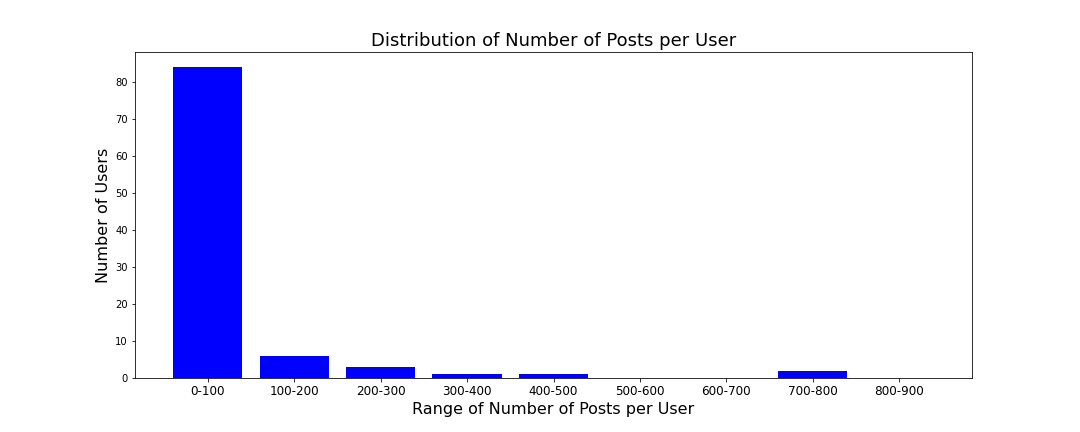
\includegraphics[width=1\linewidth]{figs/postcount1.png}}
\hfill
\subfloat[Range: 0-100] {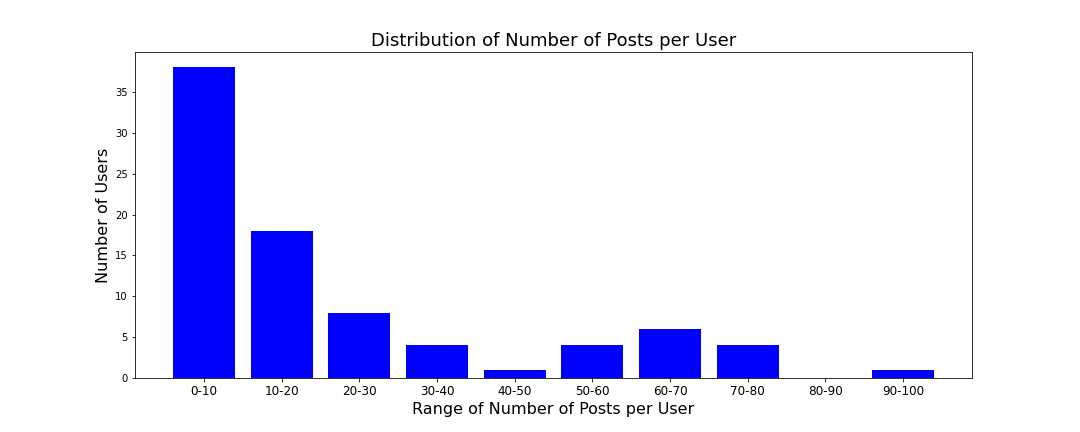
\includegraphics[width=1\linewidth]{figs/postcount2.png}}
\hfill
\subfloat[Range: 0-10] {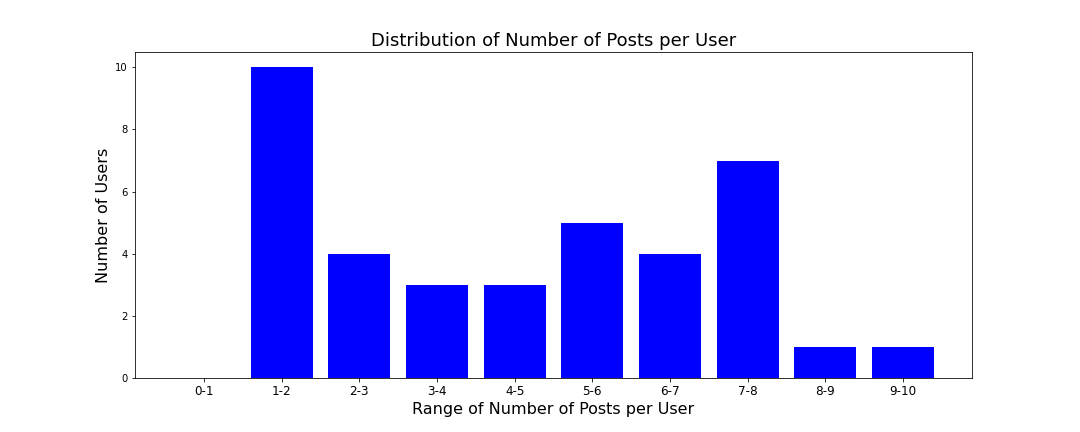
\includegraphics[width=1\linewidth]{figs/postcount3.png}}
\caption{Distribution of number or count of users with varying ranges of number of posts per user}
\label{fig:user_postcount_distribution}
\end{figure}

\subsection{Classification Model}
The first step of our analysis is to build a classification model to predict the emotion of the scraped posts. We utilize a pre-trained model\footnote{Pre-trained model: \url{https://huggingface.co/SamLowe/roberta-base-go_emotions}} for this task, specifically the model trained on the GoEmotions dataset \citep{Demszky+20:GoEmotions}. This model achieves over 0.9 accuracy in most emotions. The GoEmotions dataset is a diverse and extensive collection of text annotations, encompassing a wide spectrum of emotional categories, providing valuable insights into the nuanced expressions of human emotions in various contexts. The dataset consists of a total of 28 emotional categories, namely:


\begin{multiitem}
    \item admiration
    \item amusement
    \item anger
    \item annoyance
    \item approval
    \item caring
    \item confusion
    \item curiosity
    \item desire
    \item disappointment
\end{multiitem}

\begin{multiitem}
    \item disapproval
    \item disgust
    \item embarrassment
    \item excitement
    \item fear
    \item gratitude
    \item grief
    \item joy
    \item love
    \item nervousness
    \item optimism
    \item pride
    \item realization
    \item relief
    \item remorse
    \item sadness
    \item surprise
    \item neutral
\end{multiitem}

We use this pre-trained model to predict the emotion of each post for our Reddit user dataset. 

\begin{figure*}[h]
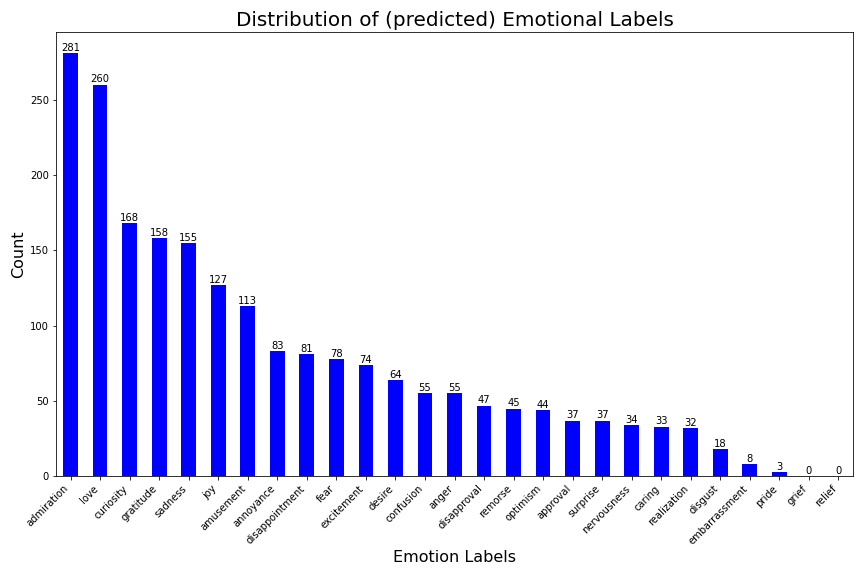
\includegraphics[width=\linewidth]{figs/emotion_distribution.png}
\caption{Count of the predicted data points for each emotion. Note that ``neutral" has been removed for better visualization}
\label{fig:emotionlabel_counts}
\end{figure*}

\subsection{Topic Modeling}
To analyze the content of posts from our Reddit User dataset, we employ topic modeling, specifically the BERTopic model\footnote{Topic modeling: \\\url{https://huggingface.co/heyitskim1912/TopicModelling}}. BERTopic leverages transformer-based language models like BERT to extract coherent topics from text data. It captures semantic relationships between words and produces interpretable topics, offering a powerful tool for uncovering latent structures within diverse textual data. To observe if contextual elements affect emotional fluctuation or if reasonable context exists beyond superficial semantics, we break down our dataset in various ways to run topic modeling. Our dataset has an 8-year gap between the oldest and the most recent posts. We divide it into four different ways: a 2-year window, a 1-year window, 30 bins, and 50 bins. Additionally, we conduct the same method on each emotion based on our predicted labels from classification. For all processes of topic modeling, we extract only nouns from the preprocessed data to get more meaningful topics, though NLTK POS tagging still recognizes some pronouns as singular nouns (e.g., im, hes, and ive). We applied bigrams and trigrams in addition to unigrams to tokenization. In addition to BERTopic, we also use LDA to compare results with BERTopic because BERTopic returns errors if tokens are not enough to interpret, while LDA even returns a topic for one sentence. 

\subsection{Word Attributions}
We utilize some model interpretability techniques to analyze the word usage or vocabulary that acts as features in the classification model while predicting. Specifically, we use integrated gradients, an explainable AI interpretability method that calculates the contribution of each input feature to a model's prediction. 

We use the \textit{transformers-interpret} Python library designed for interpreting transformer-based classification models by revealing the importance of words and phrases, allowing for a nuanced analysis of how specific vocabulary choices in Reddit posts relate to the emotional classifications assigned by our model. The library works by providing word or token-level attributions, i.e., scores of contributions of each token to each emotion, depicting the impact of individual words on model predictions, facilitates a granular analysis of feature importance. 

Combining these techniques can provide insights into the intricate connection between a user's vocabulary usage (which we assume as a part of writing style, as described in Section \ref{problem_description}) and emotional state.

\section{Emotional Analysis} \label{analysis}

\subsection{Temporal Predominant Topics Analysis}
We employed topic modeling to investigate the predominant topics and emotions over time within a specified temporal range, spanning from 2015 to the present. To get the best results for our purpose, we only use noun words present in the text, identified by NLTK. It helps to remove less significant words like pronouns. It may be risky to ignore important adjectives and verbs; however, this approach can help reduce noise and focus on the core concepts of the text.

We utilize one-year-long or two-year periods when examining dominant topics across broader time frames. Though the number of posts in earlier years was relatively low, we observed a tendency towards more general and globally relevant topics. For example, the dominant topics of postings from mid-2021 to mid-2022 are related to government and COVID-19 as shown as `globalnewsca,' `covid19,' `government,' `health,' and `leadership,' which are similarly shown in the topics derived from 2-year time frames, as shown in Table \ref{tab:2yr-topics}. 

In contrast, analyzing topics within shorter time frames revealed more personal and subjective themes. We divided time frames into 30 and 50, which means each year is divided into four to six periods. In this analysis, We got keywords like `relationship,' `wife,' `life,' `game,' `sunday,' `camera,' `work,' and `people'. Therefore, we observed that individuals delved into topics related to their relationships, interests(e.g., games), or other personal experiences.

We also conduct topic modeling for each emotion for an in-depth analysis of dominant topics. We aim to derive the relationship between events and emotions. Due to the size limitation of the dataset and its distribution, more than 3,400 data are classified as \textit{neutral}. Even though the data for each emotion is inadequate, we selected the top three most popular emotions, i.e., \textit{admiration}, \textit{love}, and \textit{curiosity}, from the classification, excluding neutral. Then, we break down the data into a 1-year window to see distribution and its topics. In Fig \ref{fig:curiosity_uni}, we observe that \textit{curiosity} peaked in 2020 with the topic `influence.' However, the results are less reliable since the other emotions do not have sufficient data for BERTopic because the tokens in the data for each emotion are insufficient for the BERTopic model. We expect to get more concrete results with larger data. To overcome this limitation, we also applied LDA, which works well with smaller token sets, to compare the results with BERTopic. With LDA, we could get more topics per bin, though the results may be less accurate than BERTopic (Fig \ref{fig:admiration}, \ref{fig:love}, and \ref{fig:curiosity}). 

As observed in Fig \ref{fig:love}, we found that the topic \textit{`im sorry'} shows up in 2020 in \textit{love}. Presumably, it has deep connections with personal loss during COVID-19 since we observed the keyword `covid19' in our temporal analysis. 

\begin{figure}[h!]
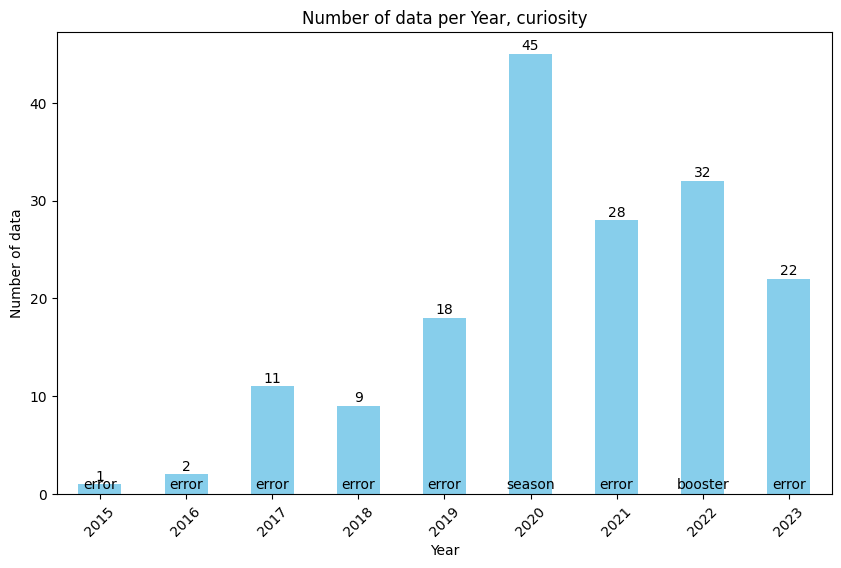
\includegraphics[width=\columnwidth]{figs/curiosity.png}
\caption{1-year window topic modeling of \textit{curiosity}. The topic of each year is marked at the bottom of each bar. `error' means there are not enough tokens for topic modeling.}
\label{fig:curiosity_uni}
\end{figure}

\begin{figure*}[ht!]
\centering
\subfloat[BERTopic-unigram] {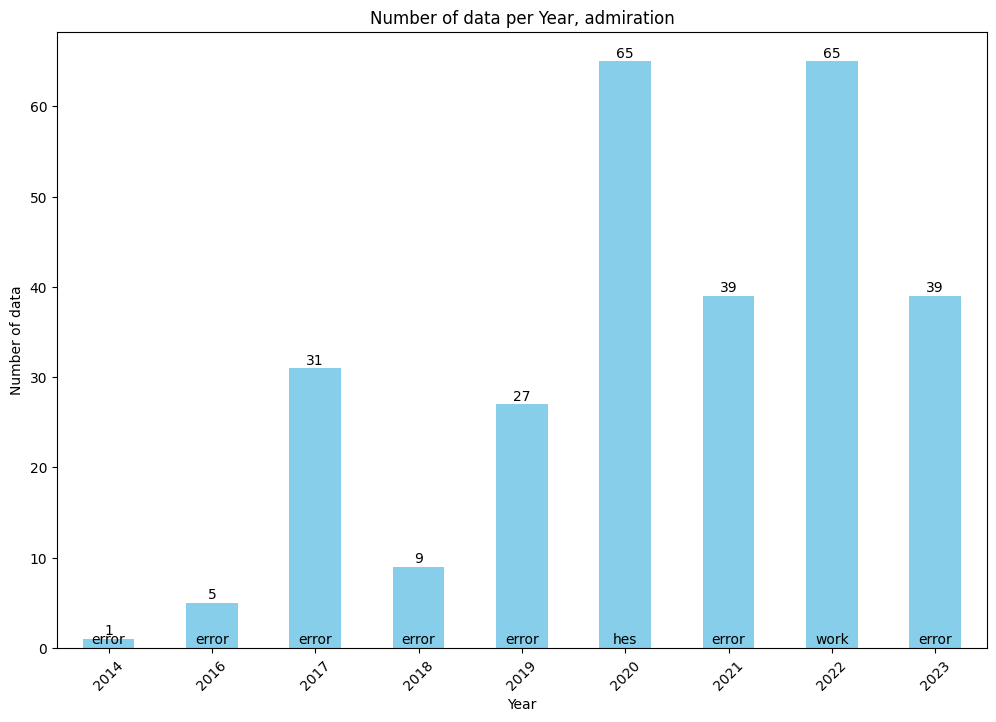
\includegraphics[width=0.5\linewidth]{figs/admiration_uni.png}}
\subfloat[BERTopic-bigram] {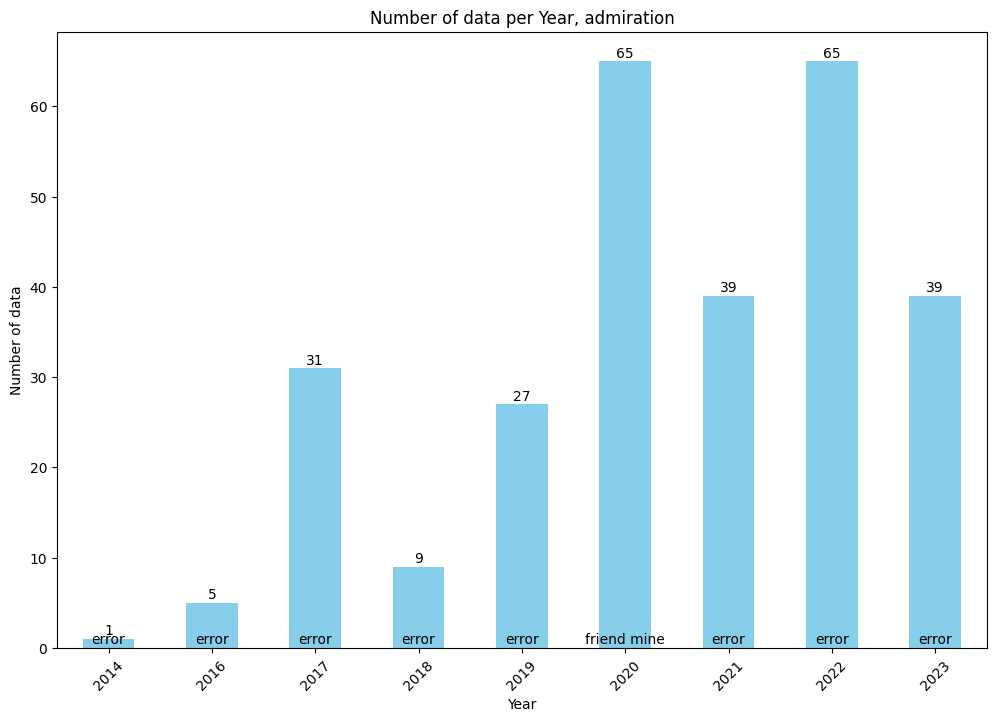
\includegraphics[width=0.5\linewidth]{figs/admiration_bi.png}}
\hfill
\subfloat[BERTopic-trigram] {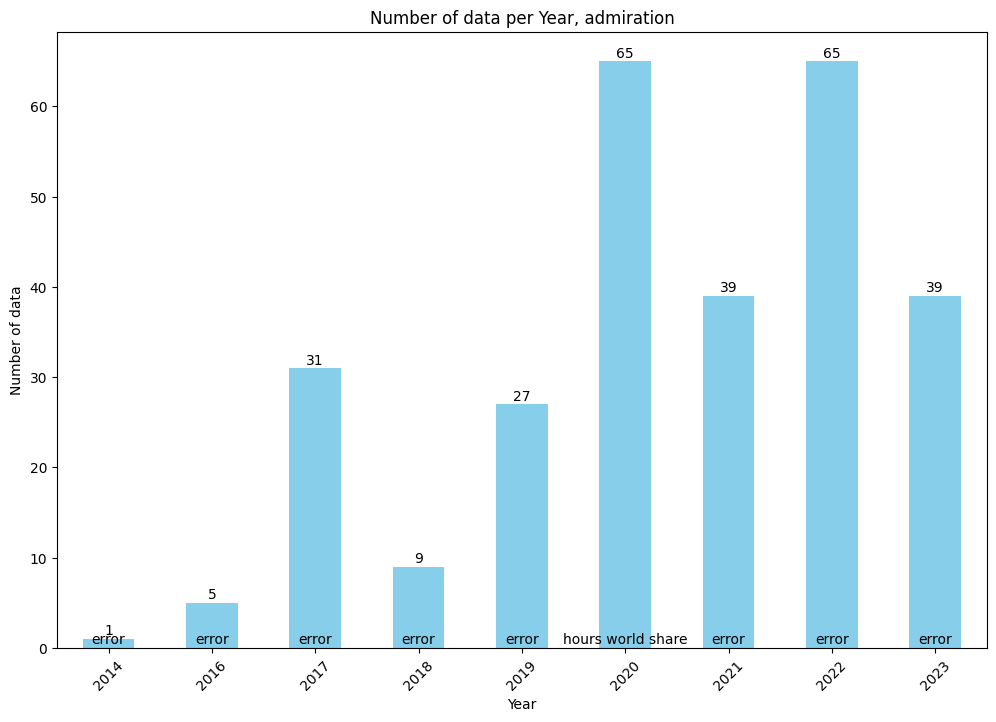
\includegraphics[width=0.5\linewidth]{figs/admiration_tri.png}}
\subfloat[LDA] {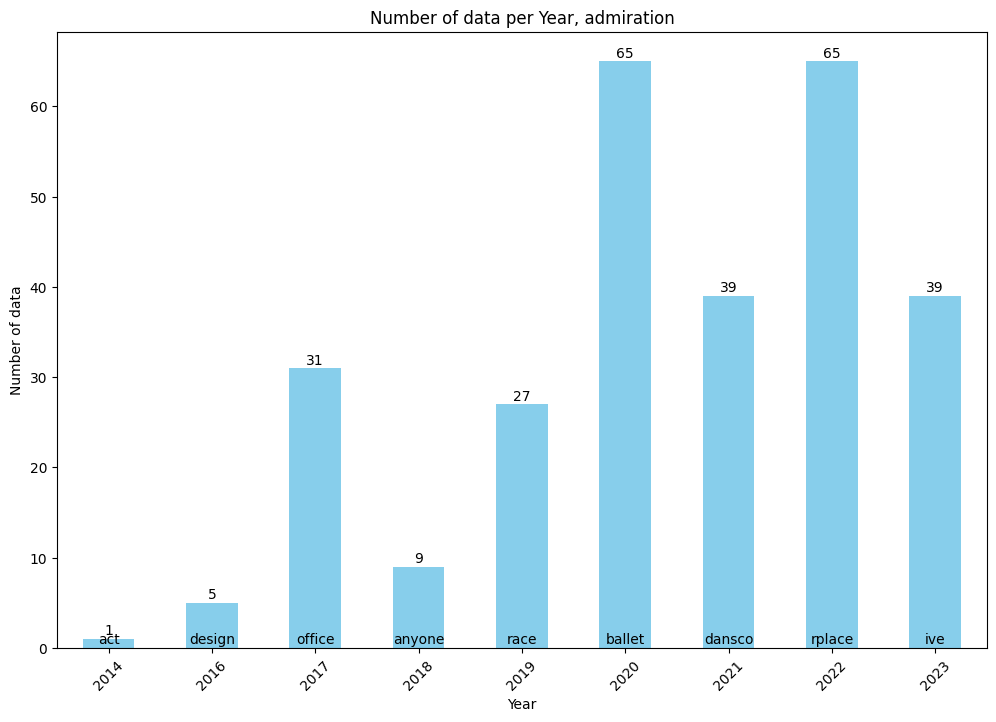
\includegraphics[width=0.5\linewidth]{figs/admiration_lda.png}}
\caption{Topics of \textit{admiration}}
\label{fig:admiration}
\end{figure*}

\begin{figure*}[ht!]
\centering
\subfloat[BERTopic-unigram] {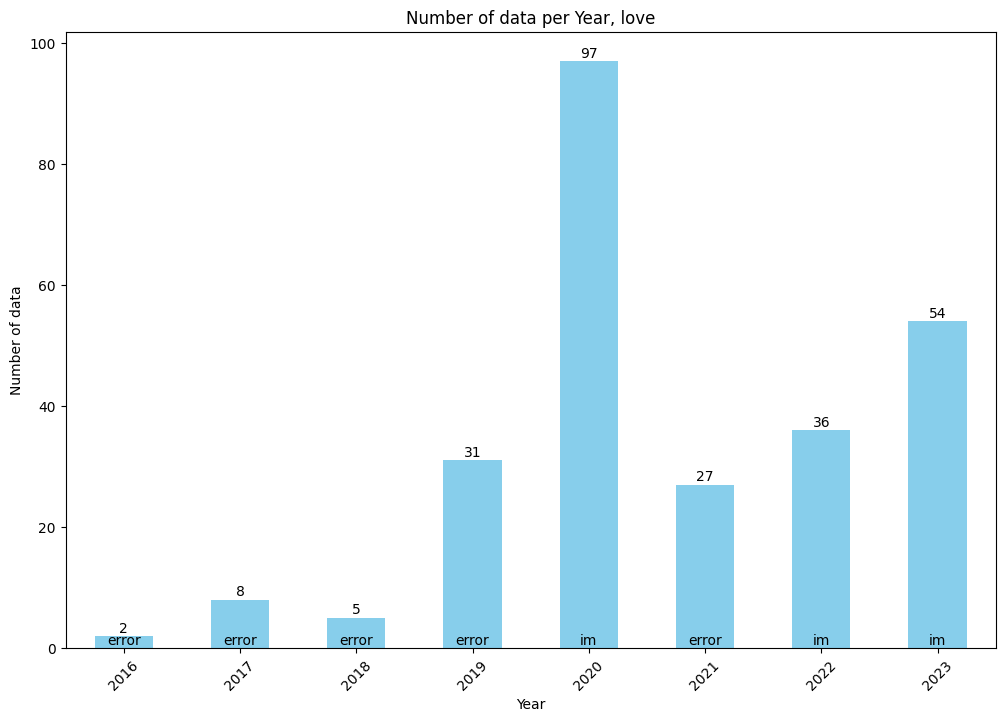
\includegraphics[width=0.5\linewidth]{figs/love_uni.png}}
\subfloat[BERTopic-bigram] {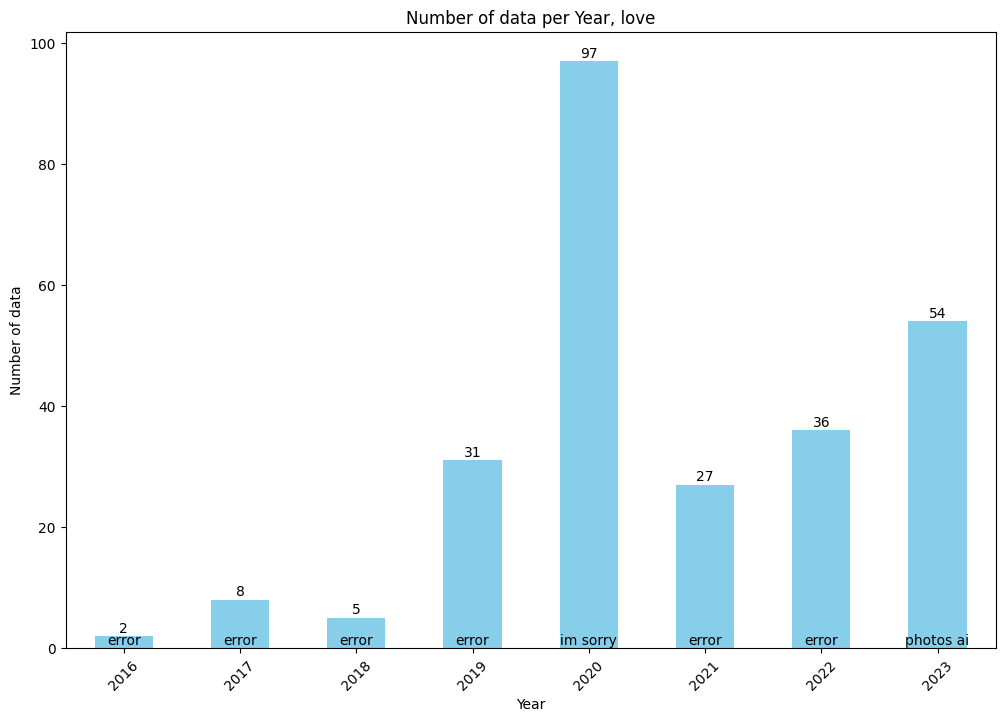
\includegraphics[width=0.5\linewidth]{figs/love_bi.png}}
\hfill
\subfloat[BERTopic-trigram] {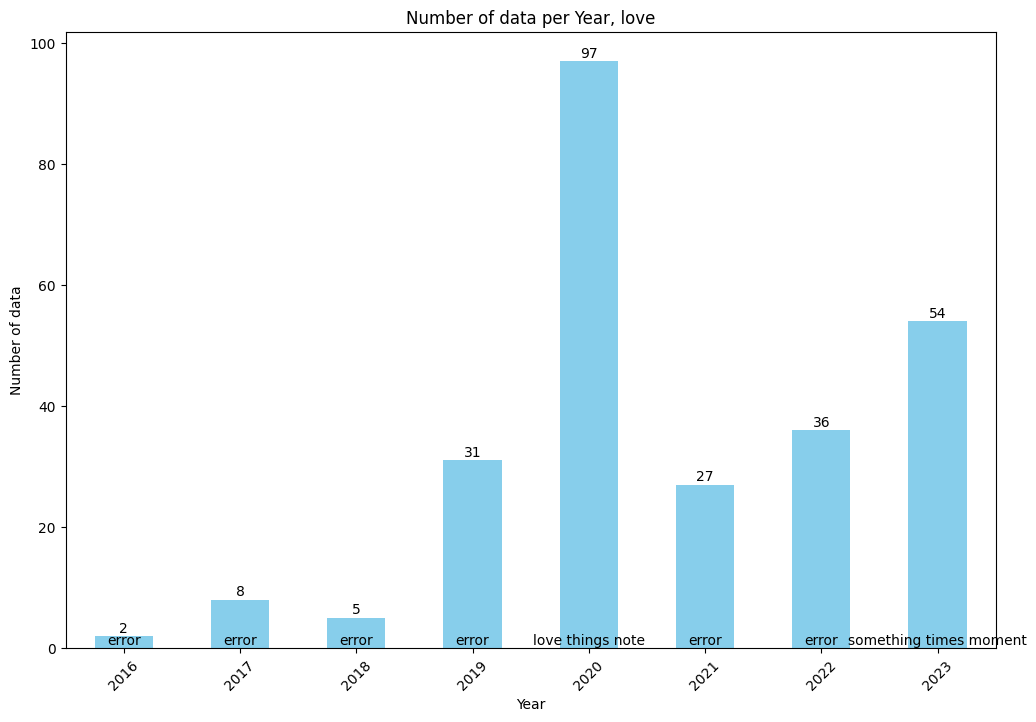
\includegraphics[width=0.5\linewidth]{figs/love_tri.png}}
\subfloat[LDA] {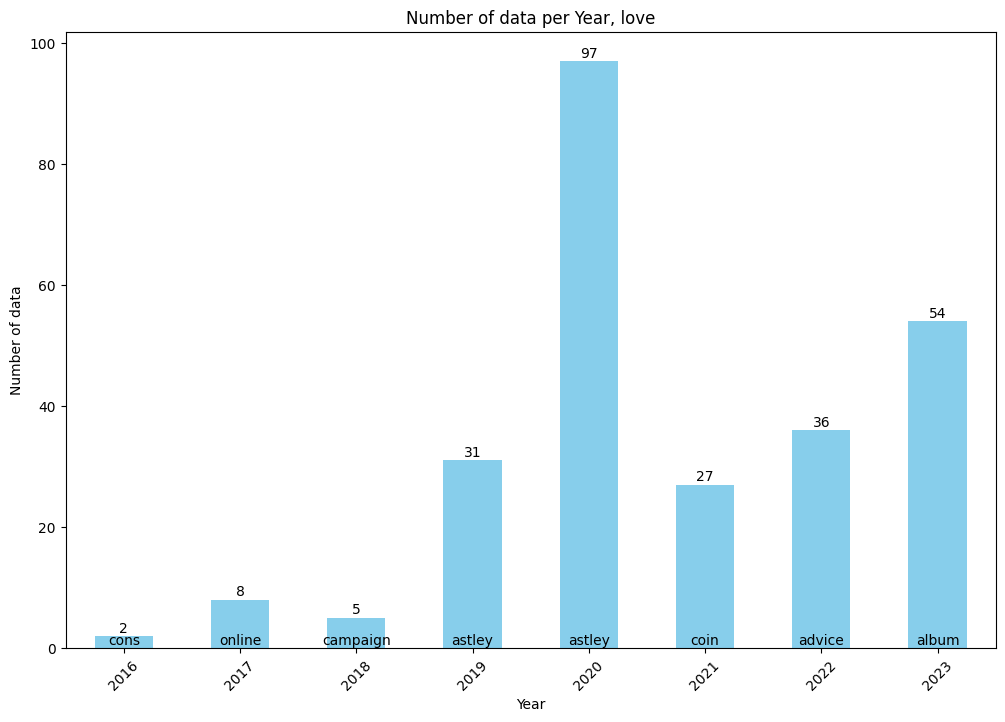
\includegraphics[width=0.5\linewidth]{figs/love_lda.png}}
\caption{Topics of \textit{love}}
\label{fig:love}
\end{figure*}

\begin{figure*}[ht!]
\centering
\subfloat[BERTopic-unigram] {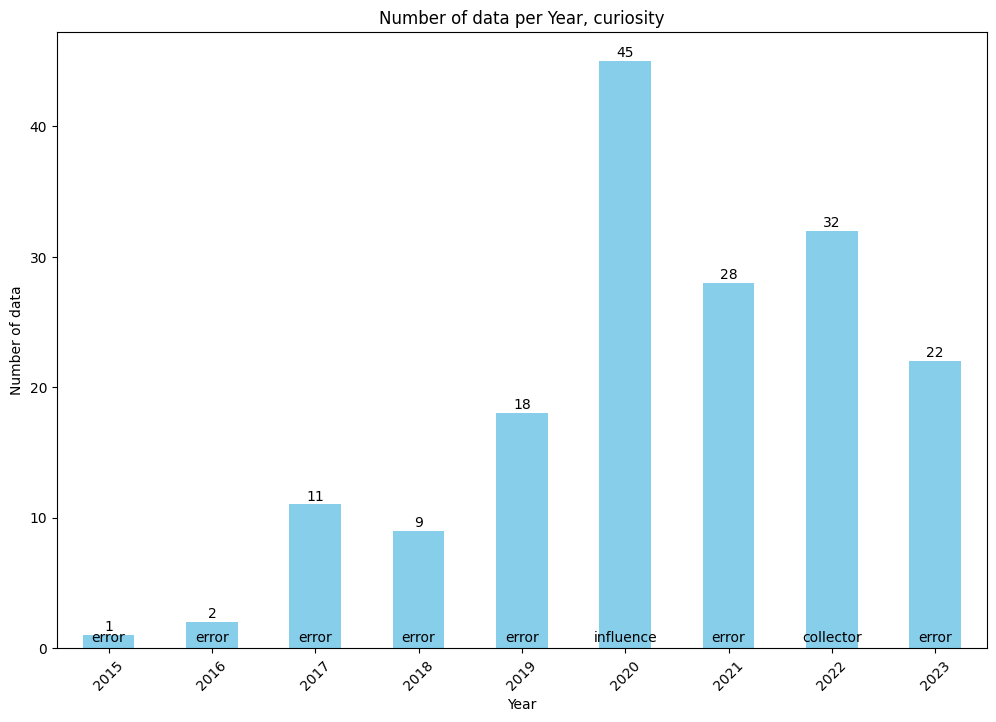
\includegraphics[width=0.5\linewidth]{figs/curiosity_uni.png}}
\subfloat[BERTopic-bigram] {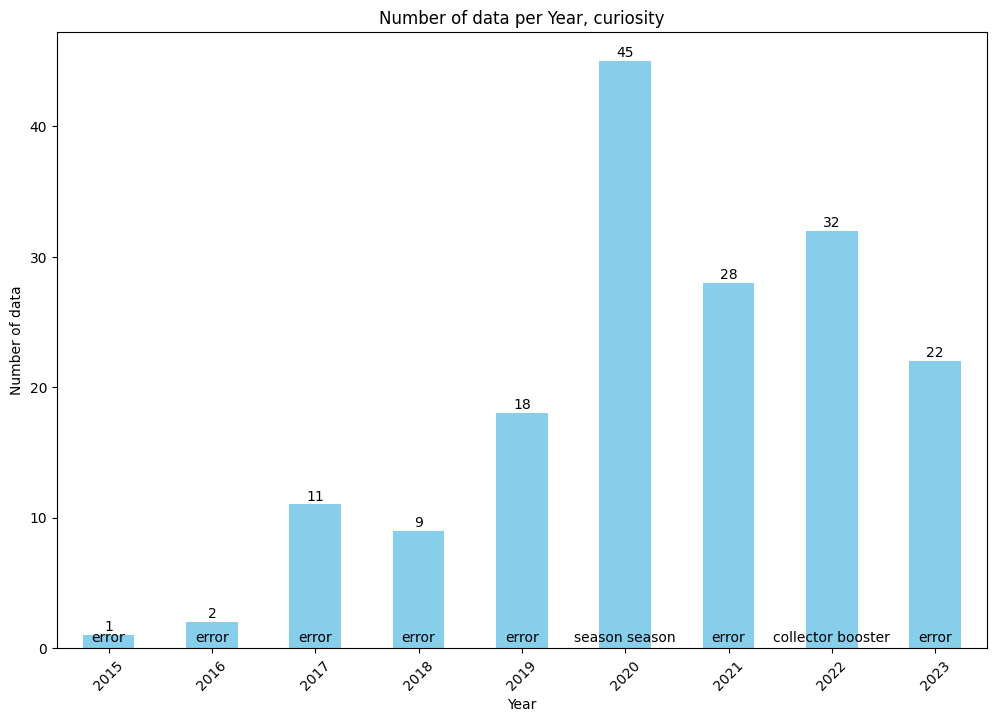
\includegraphics[width=0.5\linewidth]{figs/curiosity_bi.png}}
\hfill
\subfloat[BERTopic-trigram] {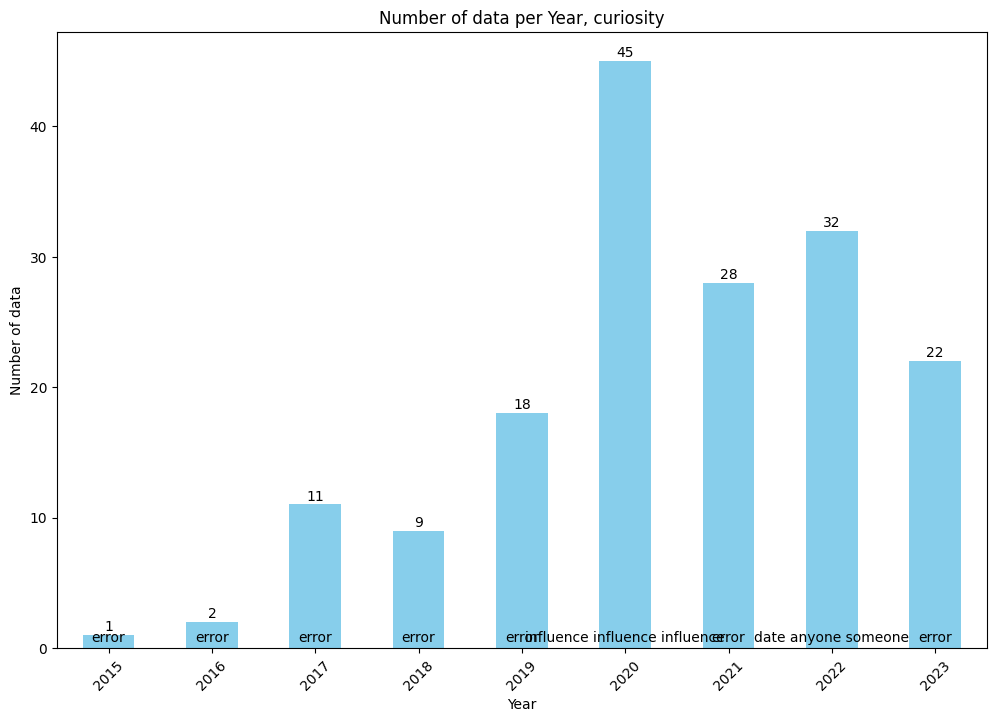
\includegraphics[width=0.5\linewidth]{figs/curiosity_tri.png}}
\subfloat[LDA] {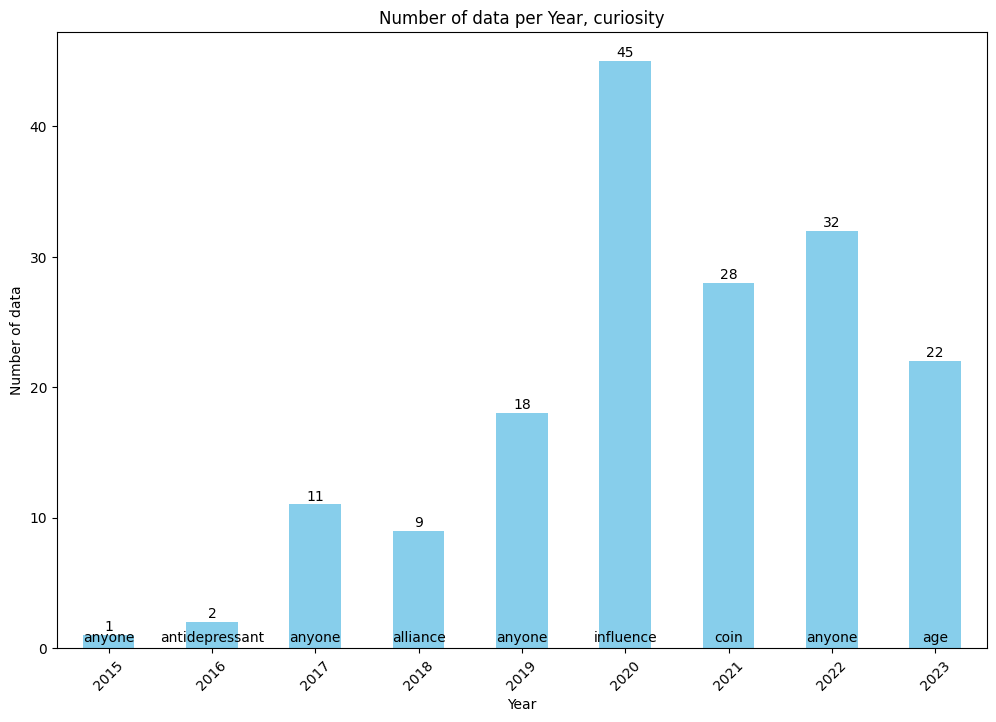
\includegraphics[width=0.5\linewidth]{figs/curiosity_lda.png}}
\caption{Topics of \textit{curiosity}}
\label{fig:curiosity}
\end{figure*}

Through this topic trends analysis, we found a potential to track individuals' life cycles and changes in emotional stages based on their life cycles. For example, teenagers might exhibit increased anxiety or stress related to their academic achievement and college admissions, while early-to-mid-30s individuals may engage in discussions about parenting, which might be linked to positive emotions such as happiness. We believe that this ability to understand individuals' emotional trends over time has the potential to provide valuable insights into human behavior and dynamics. However, our dataset may have a gender bias. Some sets of topic modeling based on time include `wife' while `husband' never appears in any of the sets. It implies that most posts in our dataset might be written by males, though ages are not remarked on. Therefore, further investigation with a larger and unbiased dataset is needed.

In addition, we observe that there is a potential to understand event-based emotional fluctuations. For example, if a certain ongoing event occurs in a specific period, it may increase a particular emotion in the crowd. It requires us to look deeply into social circumstances and remarkable events happening worldwide, matching our results. 


\subsection{Vocabulary-Emotion Relationship}

Table \ref{tab:top_words} displays the top 10 positively and negatively contributing tokens to each emotion label. To use these tokens to find a relationship between emotions, we find if some tokens overlap between two emotions, i.e., if one token is a high positive contributor to two emotions. For instance, the token ``welcome" appears in the emotions ``gratitude" as well as in ``approval." This signifies a relationship between these emotional states. We use this method to plot a graph, depicted in Fig. \ref{fig:vocab_emotion}

\begin{figure*}[h!]
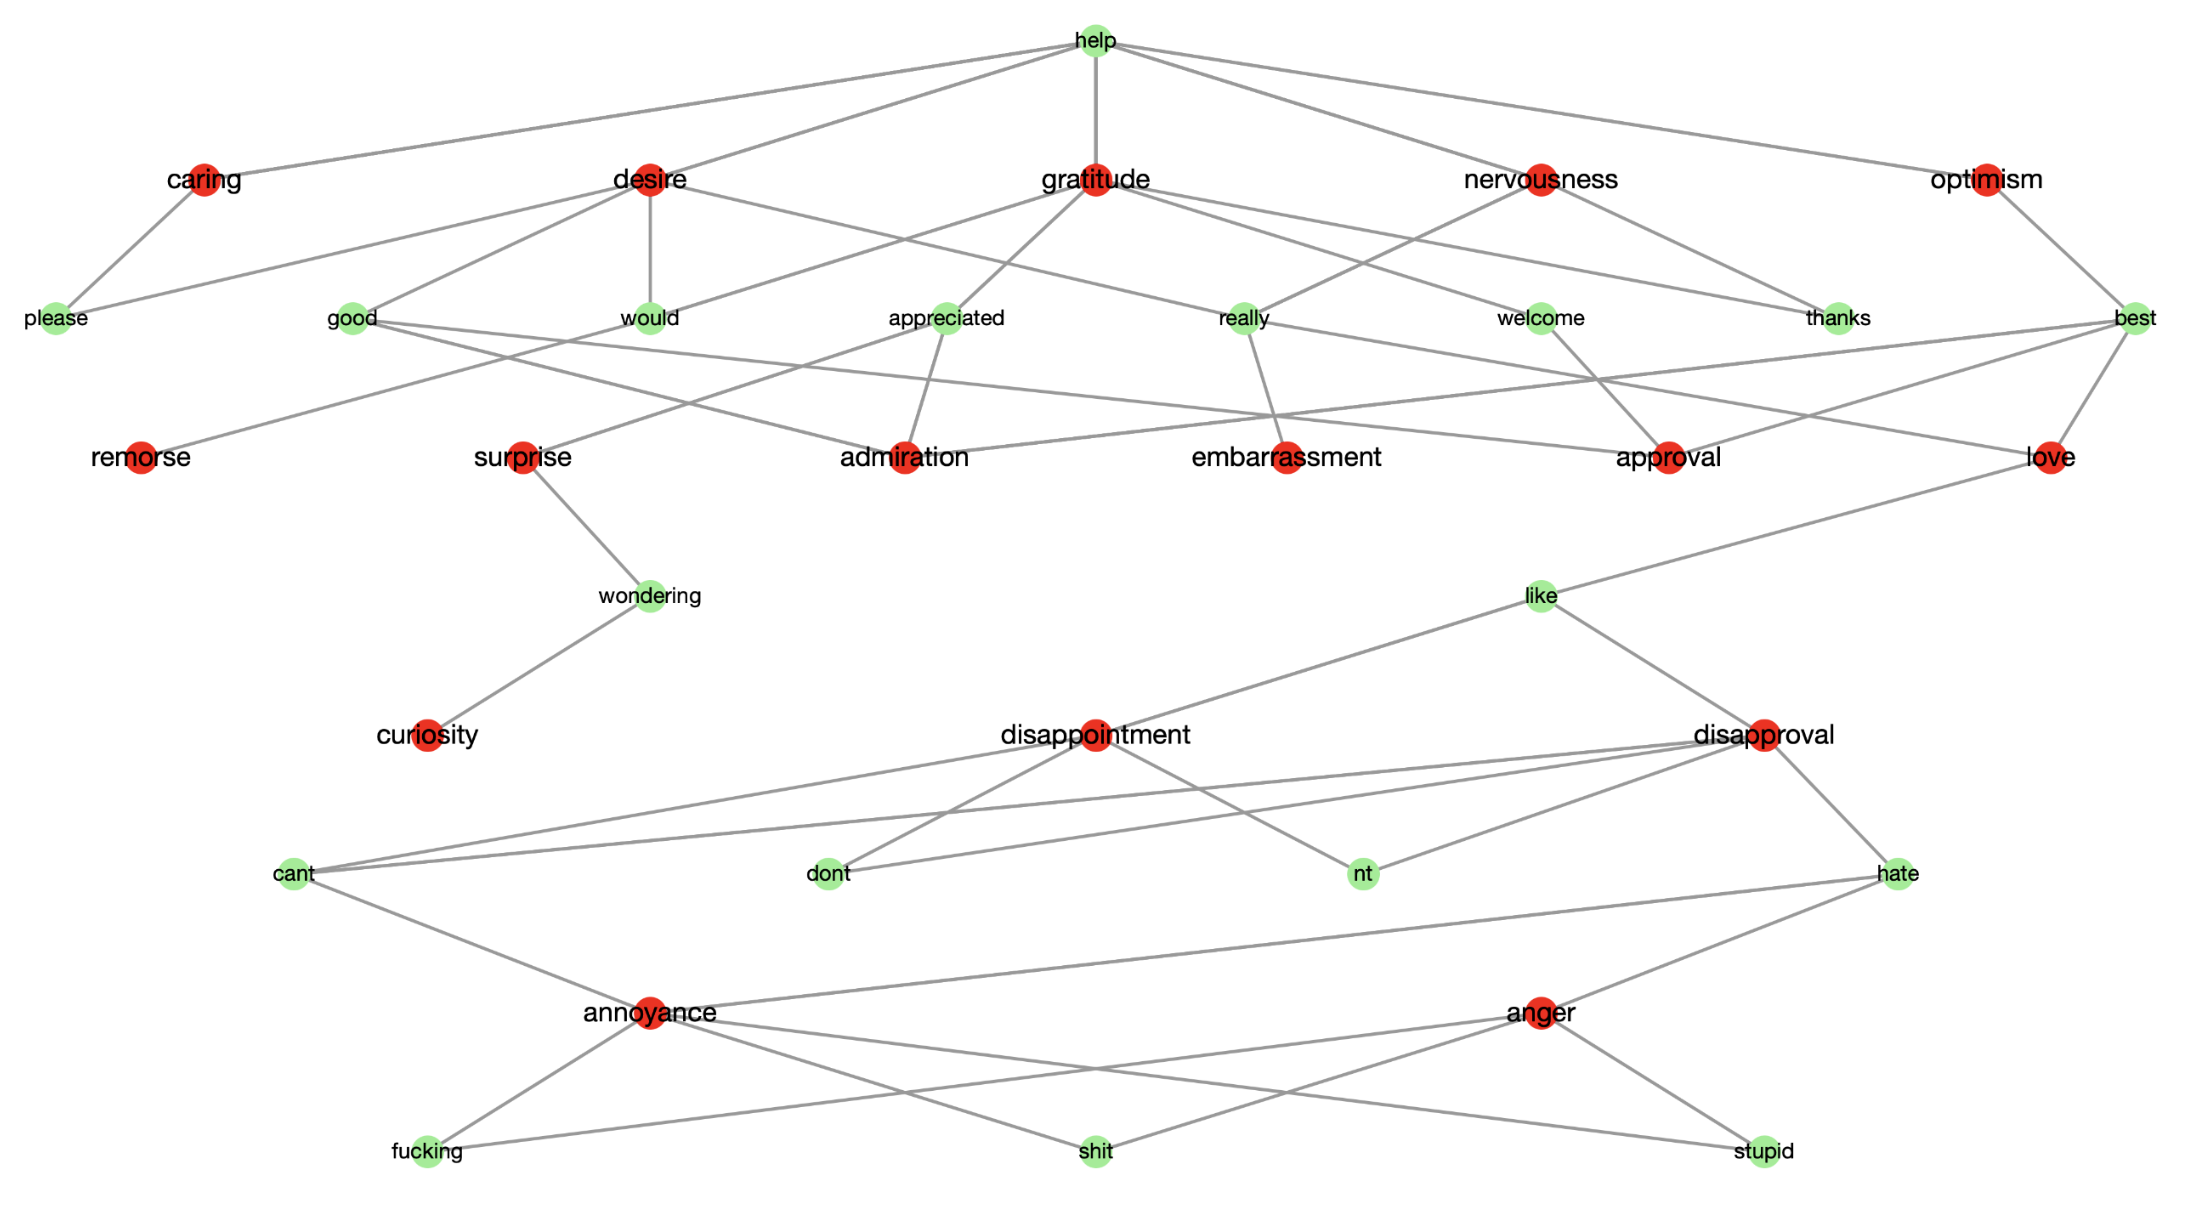
\includegraphics[width=\linewidth]{figs/vocab_emotion.png}
\caption{Graph of the Top Common Positively Contributing Words between Emotions}
\label{fig:vocab_emotion}
\end{figure*}

We can see that similar emotions tend to link together, such as \textit{disappointment-disapproval}, \textit{annoyance-anger}, \textit{surprise-curiosity}, and \textit{nervousness-embarrassment}. We also see that ``emotional fulfillment" words like \textit{caring, desire, gratitude} grouped together by the word \textit{help}, while ``affirmative sentiment" words like \textit{optimism}, \textit{love}, \textit{approval} and \textit{admiration} are linked and grouped together by the word \textit{best}.

Note that not all emotions show up since they have a distinct set of top tokens with no overlap with the top tokens of other emotions. These are \textit{amusement,  confusion, disgust, excitement, fear, joy, pride, realization} and \textit{sadness}. Interestingly, the emotions ``grief" and ``relief" do not appear in the graph. This is because, as shown in Fig. \ref{fig:emotionlabel_counts}, none of the posts are classified as these emotions; thus, no token contributes to it, i.e., their attribution score is zero towards ``grief" and ``relief." 

\subsection{Probabilistic Emotional Transitions of Users}

\begin{figure*}[h!]
{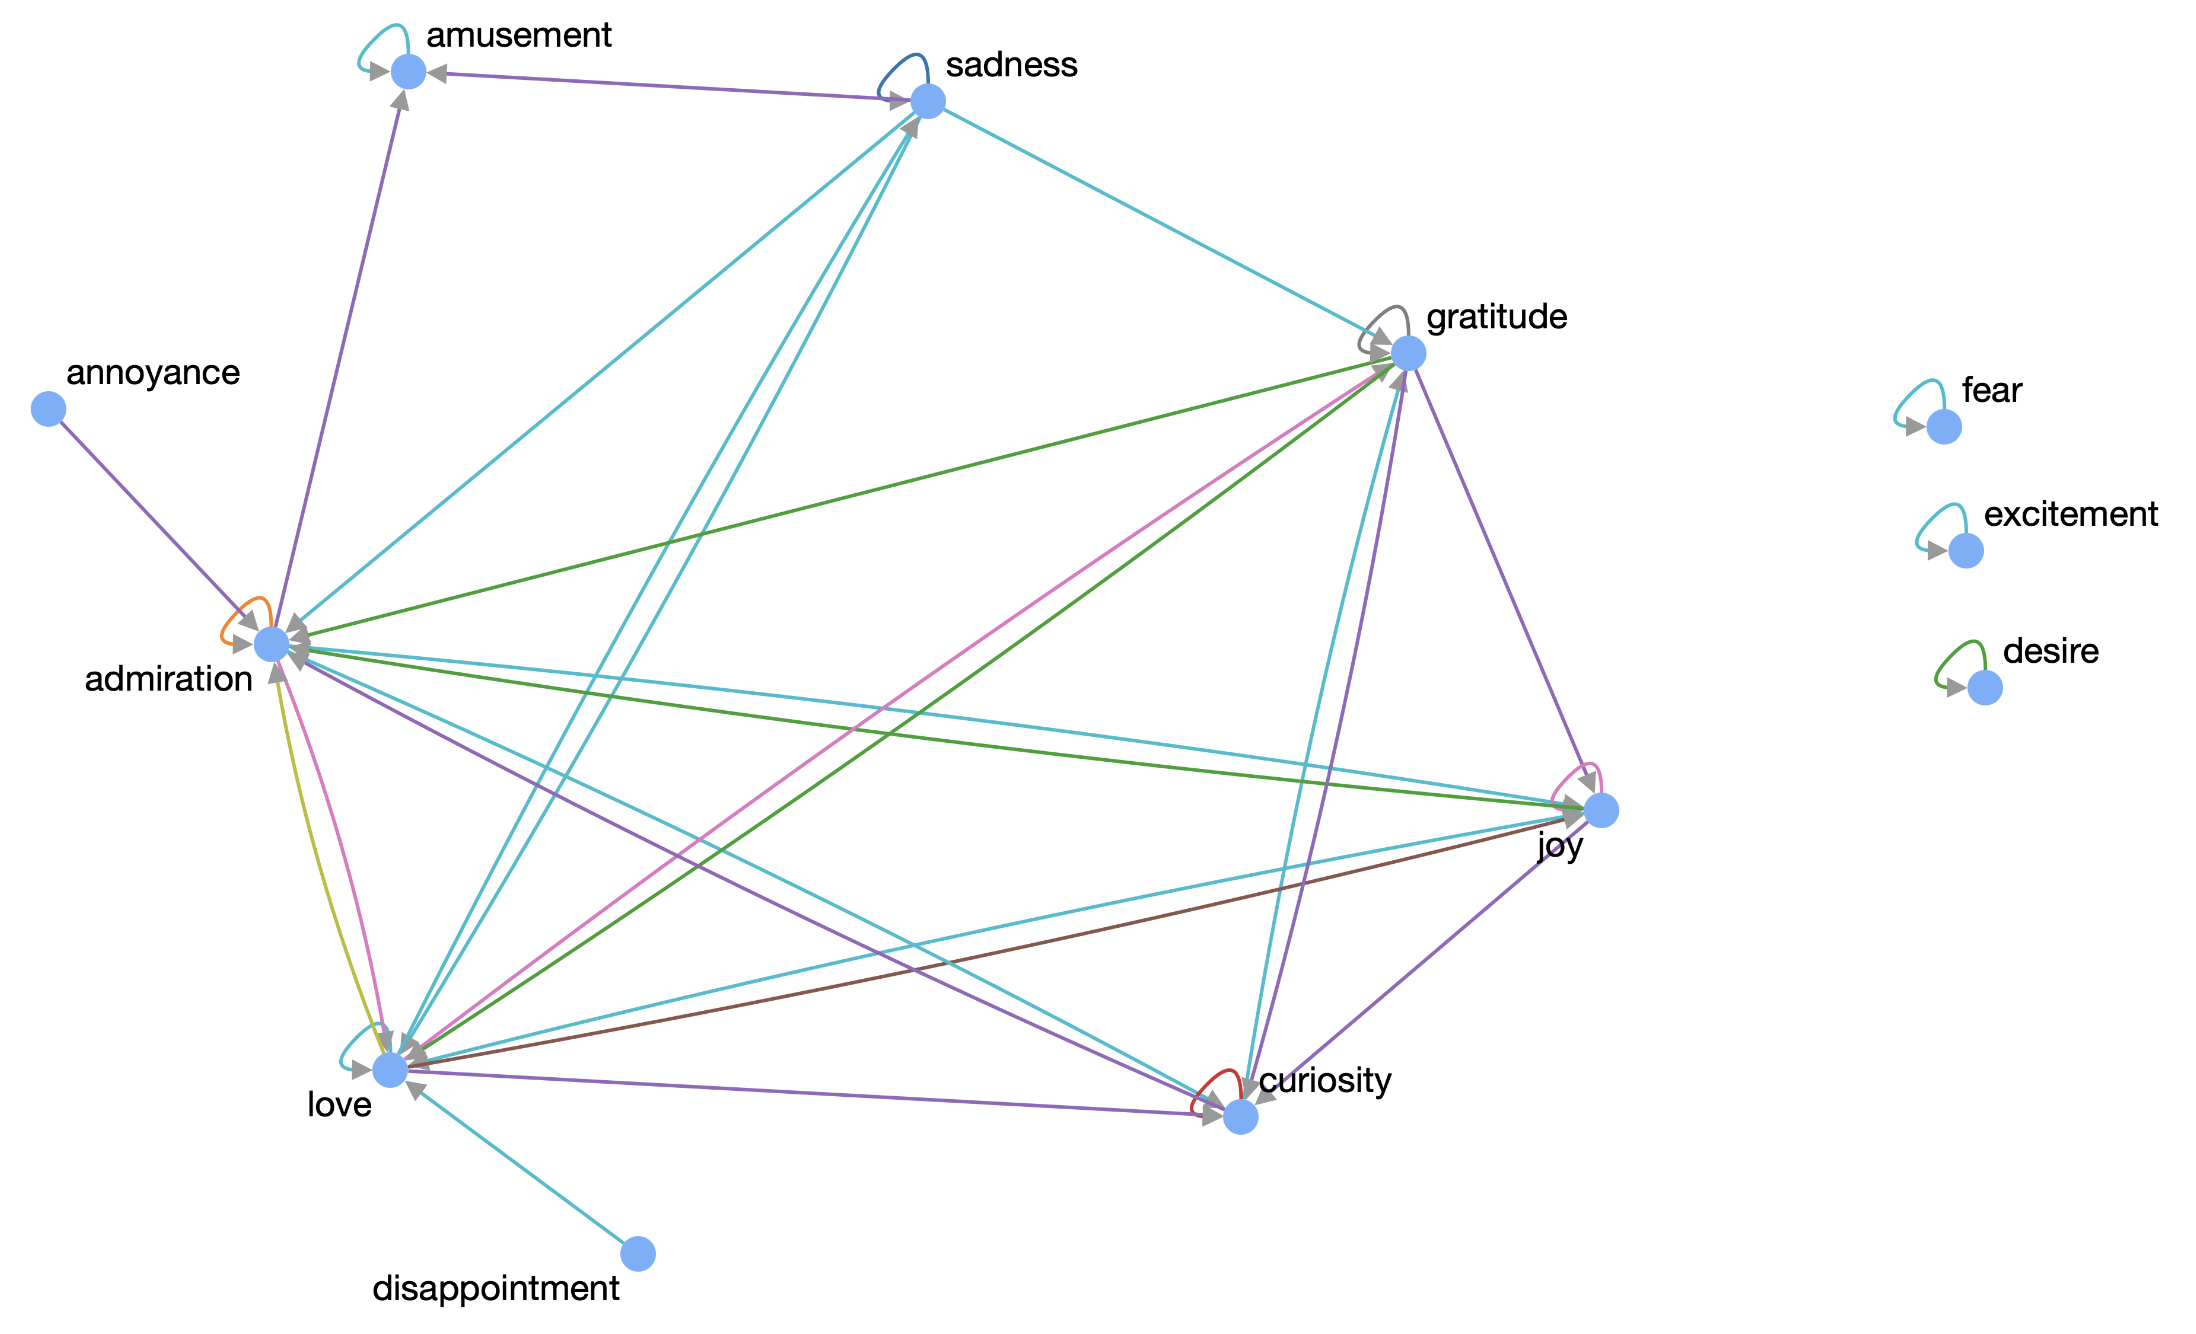
\includegraphics[width=\linewidth]{figs/lifecycle.png}}
\centering
{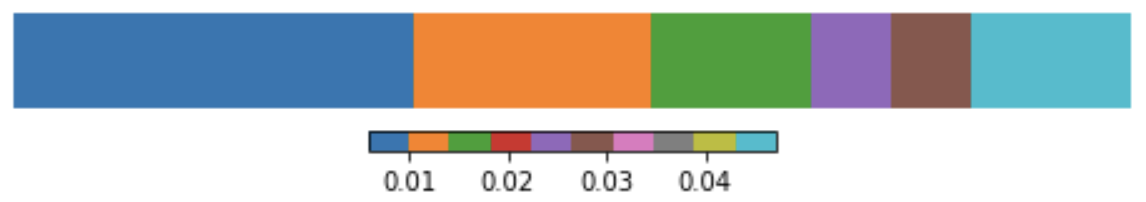
\includegraphics[width=0.6\linewidth]{figs/color_ref_lifecycle.png}}
\caption{Probabilistic emotional transitions (above 0.005) of users across their posts according to their normalized probabilities}
\label{fig:lifecycle}
\end{figure*}

A probabilistic emotional transitional model of each user refers to the emotional states a user transitions through, as identified by their Reddit posts over time. For this purpose, we compile the posts from each Reddit user chronologically and predict the emotion for each post. Thus, we get the emotional transitions of a user across his posts. We count the number of directed transitions between two emotions and find the probabilities for each transition. We then drop the probabilities involving a transition to or from the \textit{neutral} state. Finally, for the purpose of plotting, we filter out these probabilities to only use those above 0.005, normalize the probabilities, and plot them, as shown in Fig \ref{fig:lifecycle}.

We spot some patterns in this graph, such as those in the \textit{fear, excitement} or \textit{desire} state tends to continue staying in the same state, i.e., they post similar posts on Reddit. This implies that some users feel continuous \textit{fear}, which could be a sign of concern. A mental health community can intervene at such a step to provide assistance. This also applies to a user feeling \textit{desire}, since it implies that they might be unhappy with their current lifestyle and always desire more.

It is interesting to note that not all emotions have self-loops. We also see a direct transitions like $\textit{disappointment} \rightarrow \textit{love}$, $\textit{annoyance} \rightarrow \textit{admiration}$, or $\textit{sadness} \rightarrow \textit{admiration, love, gratitude}$ which can be inferred as an emotional transition from a negative emotion to a positive emotion.

The highest probability emotional transitions are the self-loop on \textit{admiration} and \textit{curiosity}. This could be attributed to the imbalance in the emotional label counts in our dataset. 

Thus, the graph captures the user's emotional journey, showcasing patterns, recurrences, and the sequence of emotional states. Such a visualization provides a comprehensive depiction of how emotions interconnect and change over time, offering a graphical narrative of the user's emotional experience on Reddit.

\section{Alternative Approaches}
In the process of performing our analysis, we encountered a few alternative approaches. 
The overall problem of mapping transitions in writing style to transitions in emotions, as shown in Fig \ref{fig:lifecycle} can also be performed by clustering the GoEmotions dataset to achieve writing style clusters based on the algorithms that define stylometry, such as \textit{Hapax Legomenon} and \textit{Hapax DisLegemena} for indicating word uniqueness, and \textit{Honores R Measure} and \textit{Sichel’s Measure} for assessing lexical diversity. We would then predict which writing style cluster each Reddit user's post would fall into and if that provides us with any assistance in predicting their emotion. However, this approach is less feasible since the GoEmotions dataset consists of 58k Reddit posts, so obtaining these linguistic features is extremely time-intensive. Our approach of computing integrated gradients to obtain user vocabulary and performing topic modeling to obtain user post content has a runtime that is approximately 2000 times faster, despite its limitation with defining writing styles. 

Among the model interpretability libraries, we decided to leverage the \textit{transformers-interpret} library since it runs well for transformer-based models, its ability to work on textual data, its ease of usage, and its fast runtime, unlike libraries ``AllenNLP Interpret," ``Captum," ``SHAP (SHapley Additive exPlanations)," ``InterpretML" and ``XAI." 

There are also some alternatives to our method of deriving the predictions of emotions for each post. We encountered pre-trained models ``MentalBERT" and ``MentalRoberta" \citep{Ji+21:MentalBERT}. However, these models were fine-tuned for mental health disorders and are thus biased toward them. It makes those models unfit for our Reddit User dataset, which is more general.

We also encountered the \textit{``joeddav/distilbert-base-uncased-go-emotions-student"} model. However, it is inferior in comparison to our chosen \textit{``SamLowe/roberta-base-go\_emotions"} model. This is due to a few reasons. One drawback of the DistilBERT model is that it is distilled from a zero-shot classification pipeline on the unlabeled GoEmotions dataset, which may result in performance limitations compared to models trained with full supervision. In contrast, the Roberta-base model benefits from being directly trained on the GoEmotions dataset, allowing for better performance in multi-label classification tasks. Additionally, the availability of an ONNX version for the Roberta-base model enhances its inference speed and reduces dependency size, making it more versatile and efficient for various deployment scenarios.

Our chosen topic modeling model, ``BERTopic" is often considered more reliable than traditional topic modeling models like Latent Dirichlet Allocation (LDA) due to its use of pre-trained BERT embeddings. By leveraging BERT's contextual understanding of language, BERTopic captures nuanced relationships in the text, leading to more accurate topic representations. This enhanced reliability is particularly beneficial in tasks requiring precise interpretation. However, the increased computational demands of BERTopic may affect its speed compared to simpler models like LDA or Non-Negative Matrix Factorization (NMF). We tackle this issue by leveraging GPU-accelerated processing power. 

\section{Evaluation}

\subsection{Evaluation on the Hypotheses}

\begin{itemize}
    \item \textbf{H1: Connection between word usage and emotional shifts} \\
    Our initial hypothesis mentions that there is a correlation between the vocabulary, or the word usage of a user, and his emotional state. Our analysis confirms our results to some extent, where we see similar emotions link together by common words. However, we have low confidence in the classification model and our dataset due to the several factors mentioned in Section \ref{limitaion}. Thus, this is still a topic to be investigated further with a richer dataset and a more accurate and reliable model. 

    \item \textbf{H2: Impact of external context on emotional shifts} \\
    We initially assumed that external factors like significant events or prevalent global phenomena could influence emotional shifts, even in age-specific contexts. Since individuals are not isolated but interconnected within a society, external factors definitely affect the formation of an individual's emotions. To examine this hypothesis, we utilize topic modeling techniques to obtain a comprehensive analysis; as a result, the findings indicate a potential association between events and emotional fluctuations despite the constraints of data availability. Specifically, we observe instances where specific events, such as COVID-19, appear to coincide with topic modeling. Similarly, we imply that the pervasive situation during COVID-19 affected having `im sorry' in the peak of \textit{love} emotion topic analysis. While our result did not provide definitive proof of a causal relationship, the observation reveals the potential impact of external factors on emotional shifts. 

\end{itemize}

\subsection{Evaluation on Methods}
Fig. \ref{fig:WA-examples} shows some examples of example sentences from the dataset with tokens displayed in green if it is a positive contributor, red if it is a negative contributor, and white otherwise. We see in \subref{wa-a} that the model correctly predicts the emotion of the post and the highlighted words in green that contribute to the prediction. \subref{wa-b} shows that the model incorrectly predicts the label since the sentence contains the token ``sorry", highlighted in opaque green, thus heavily influencing the prediction. \subref{wa-c} shows a correct prediction of neutral with tokens highlighted in red and green. \subref{wa-d} shows a counter-example of \subref{wa-b} where the emotion occurring in the text is the accurate prediction. 

\begin{figure*}[ht!]
\centering
\subfloat[Positive Example] {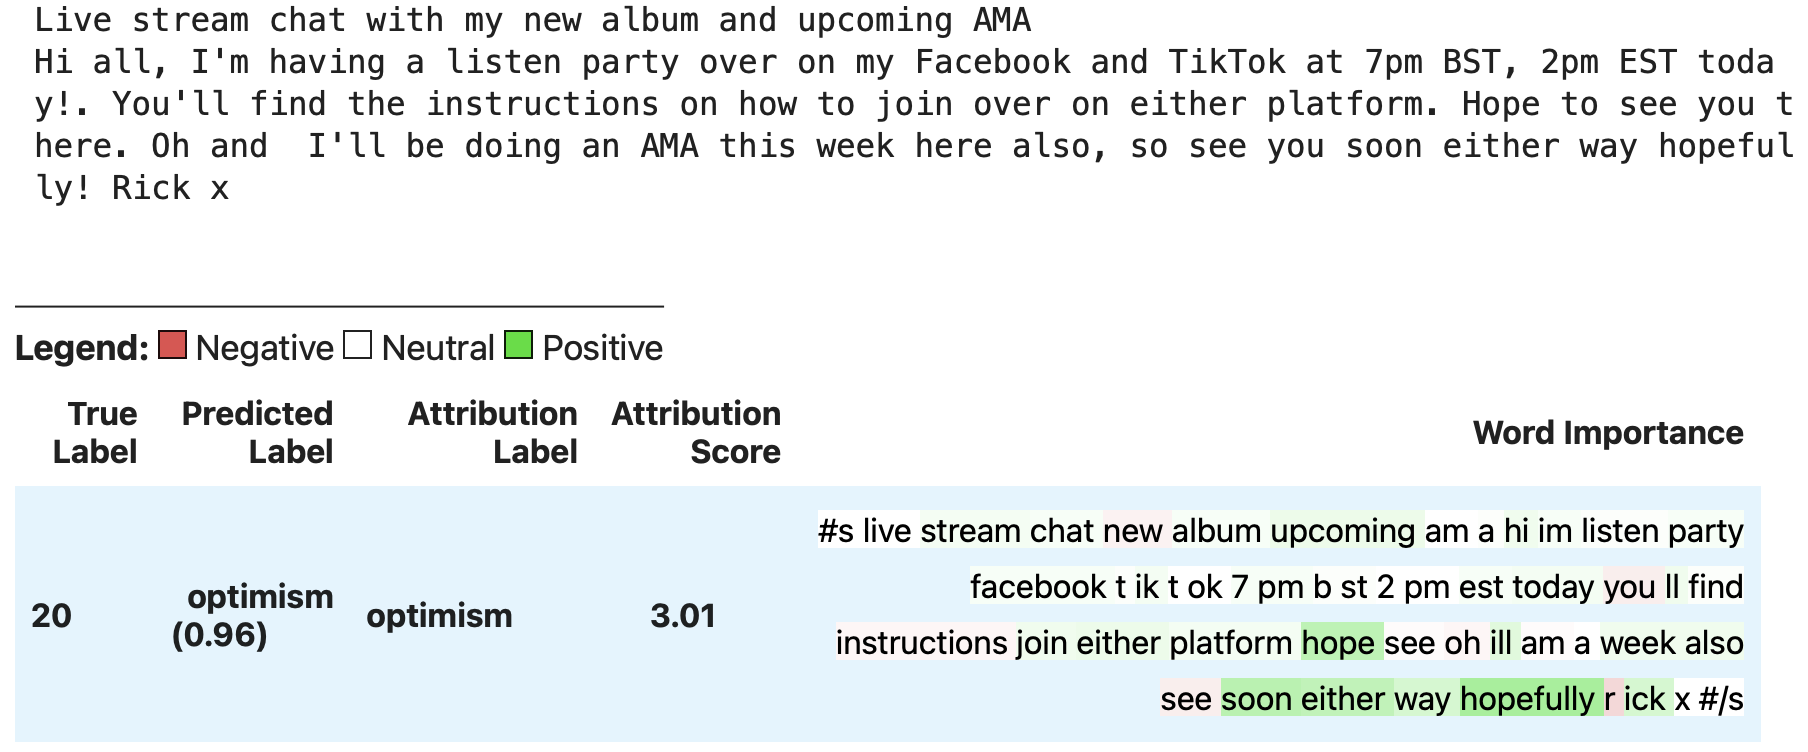
\includegraphics[width=0.5\linewidth]{figs/eg1.png}\label{wa-a}}
\subfloat[Negative Example] {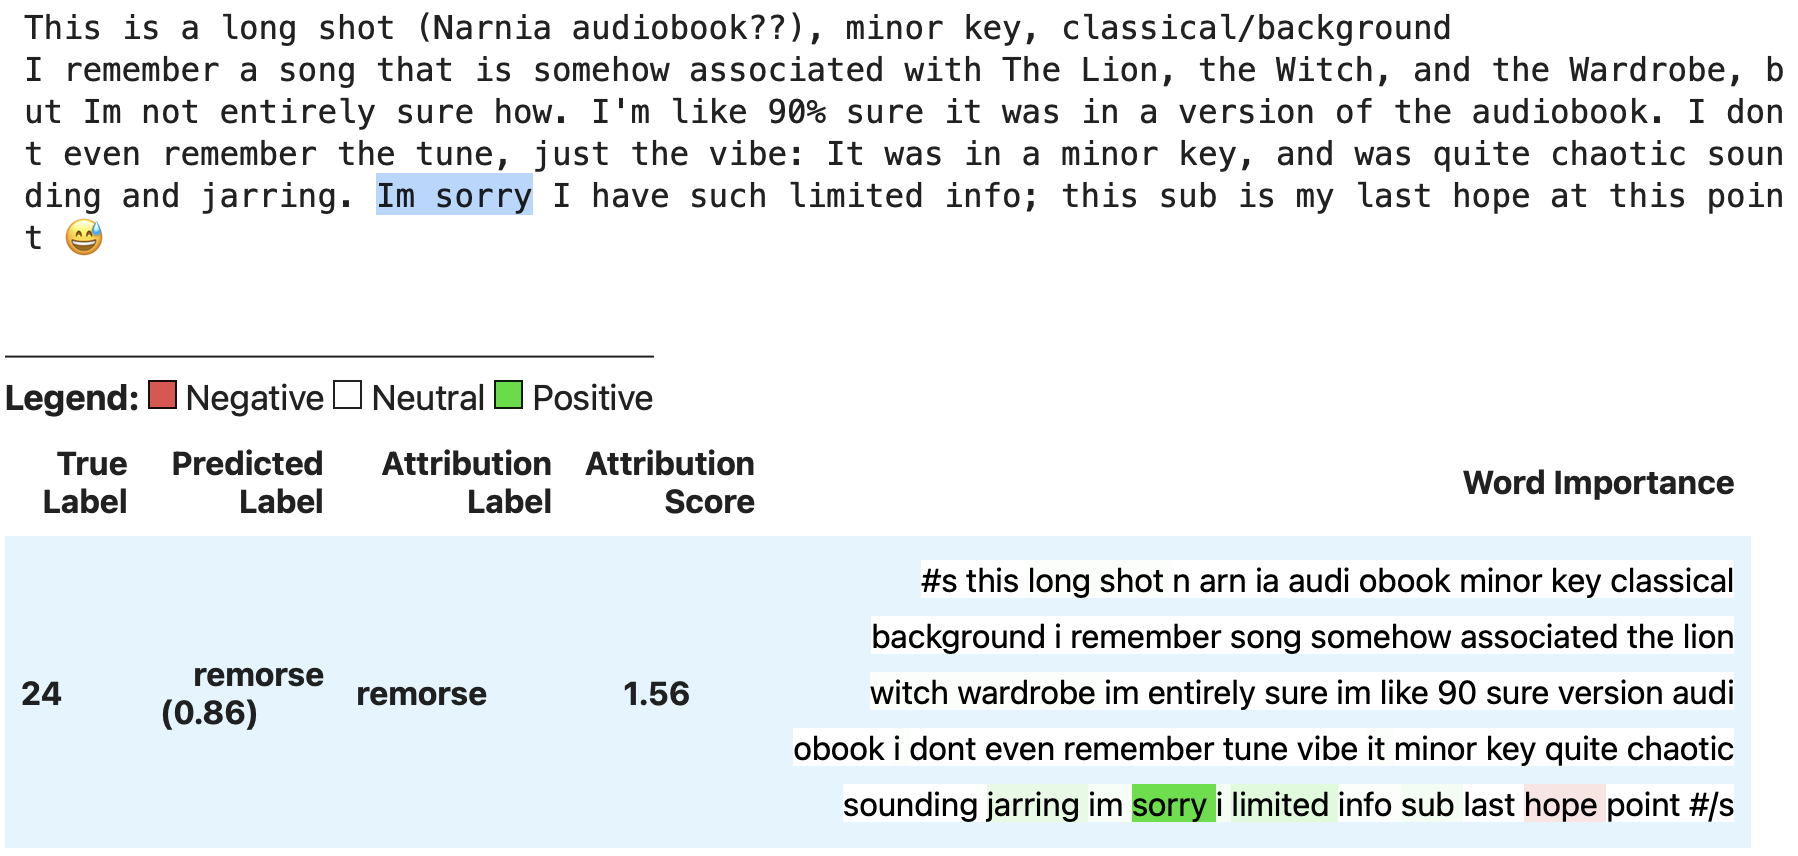
\includegraphics[width=0.5\linewidth]{figs/eg2.png}\label{wa-b}}
\hfill
\subfloat[Positive Example] {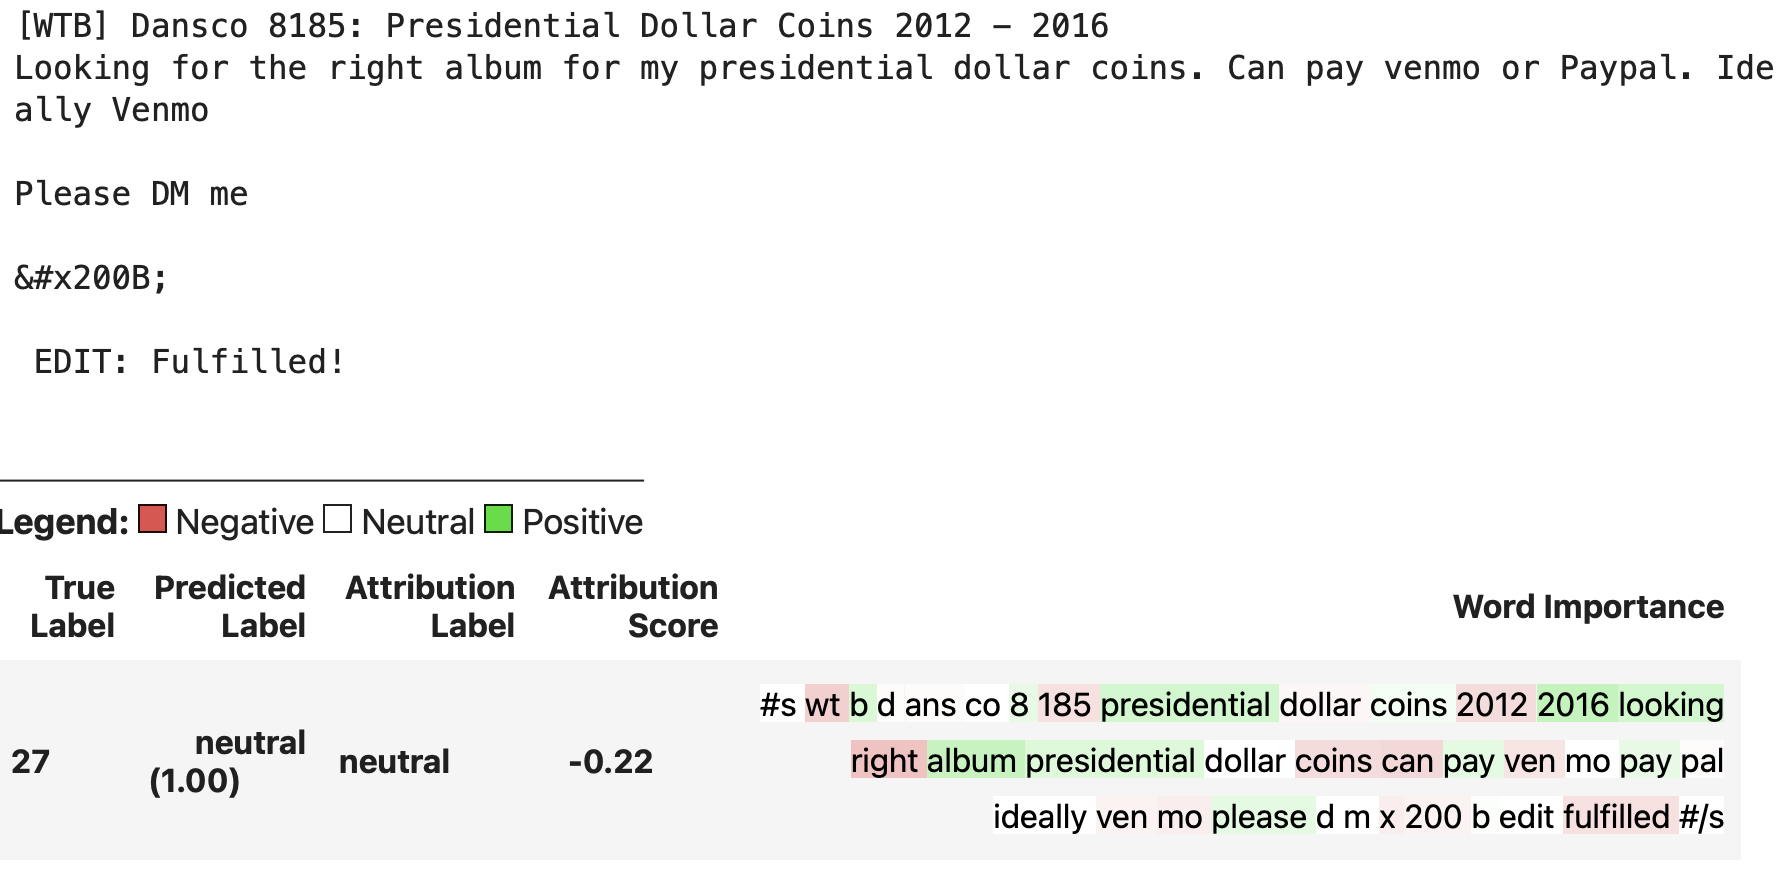
\includegraphics[width=0.5\linewidth]{figs/eg3.png}\label{wa-c}}
\subfloat[Positive Example] {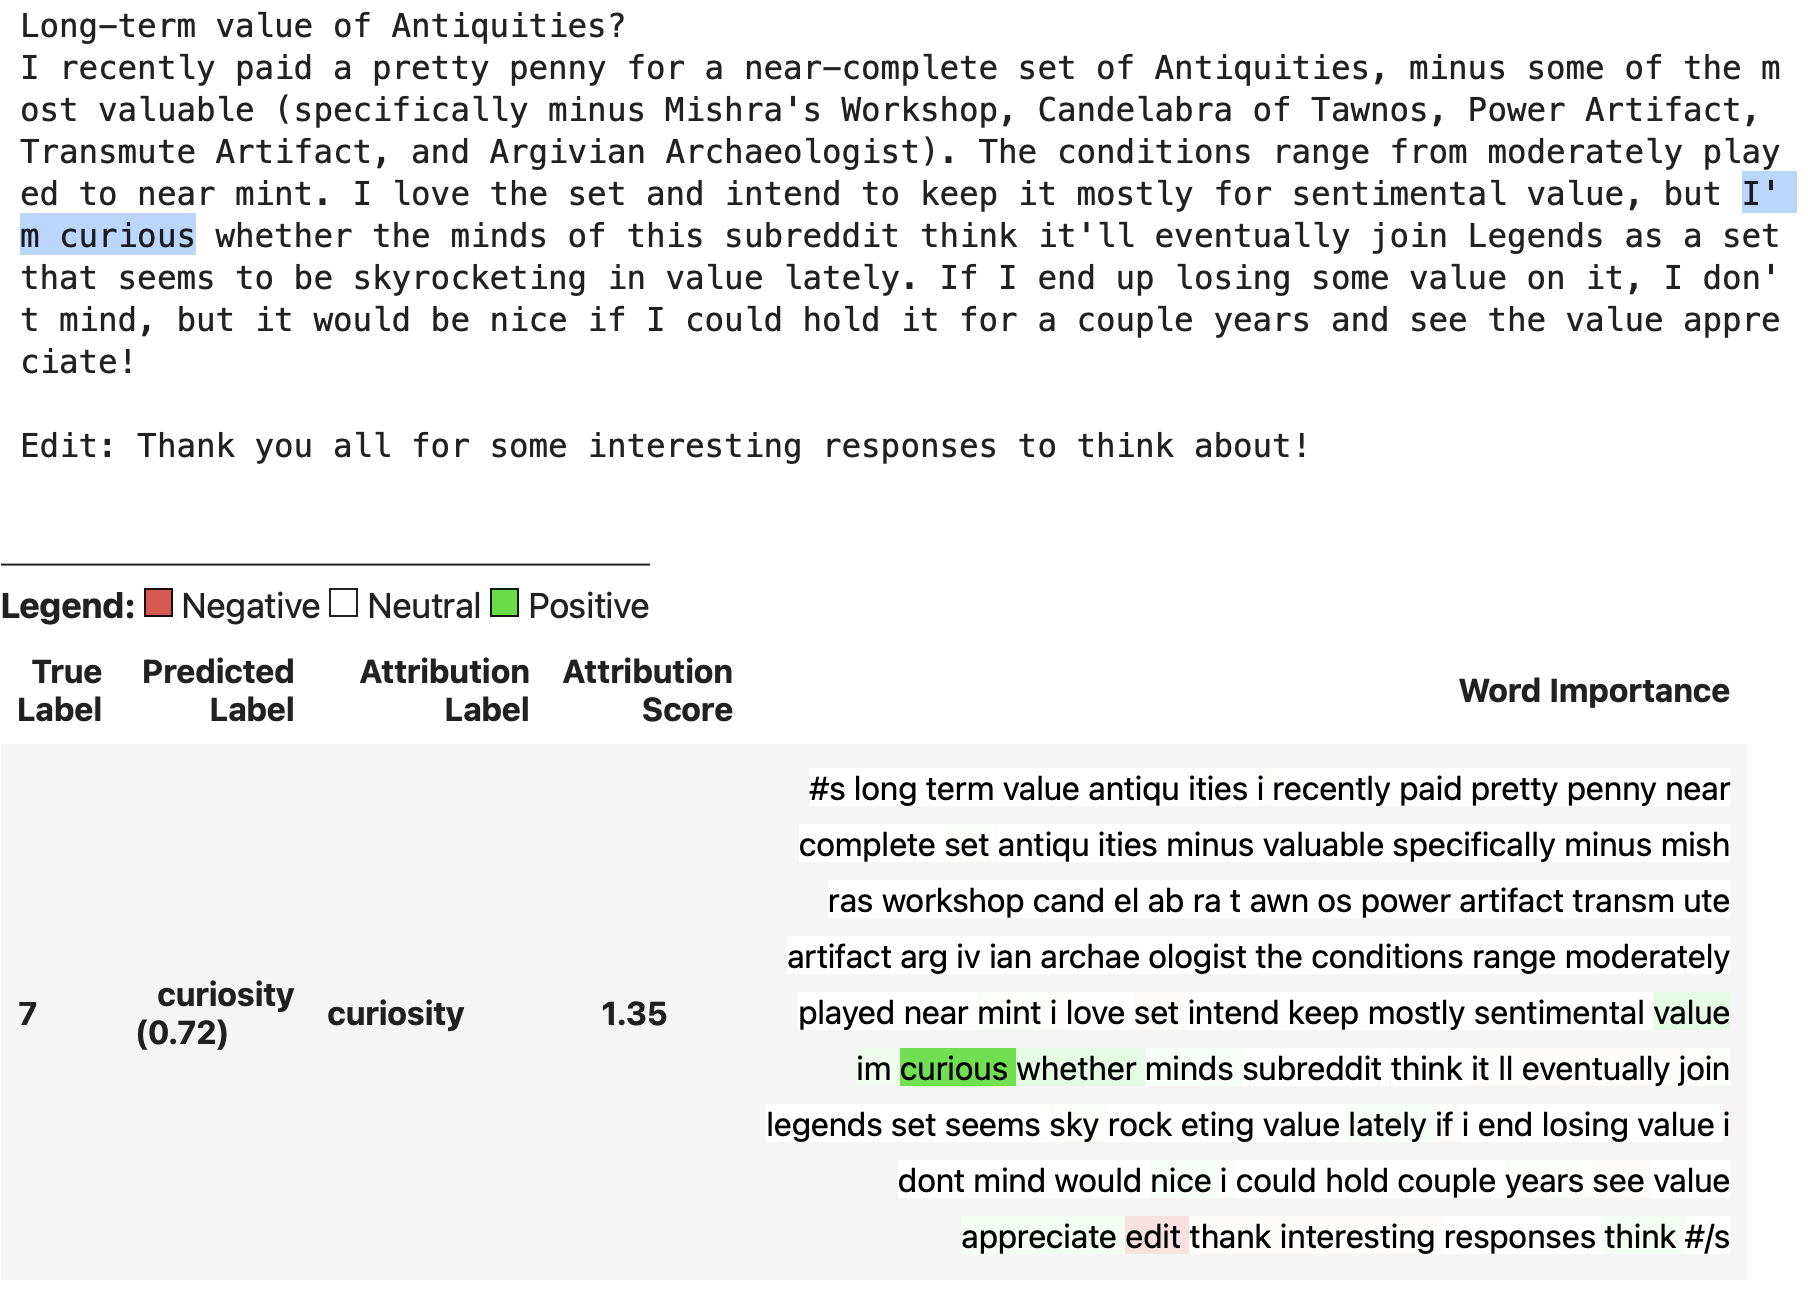
\includegraphics[width=0.5\linewidth]{figs/eg4.png}\label{wa-d}}
\caption{Examples of classification model and word attributions}
\label{fig:WA-examples}
\end{figure*}


\section{Main Findings}

Our main findings, as discussed in detail in Section \ref{methodology} and \ref{analysis}, have been summarised below. 

\subsection{Temporal Predominant Topics Analysis}
\begin{itemize}
    \item Macro-scope temporal analysis like one-year-long or 2-year-long reveals more general and broader topics that may be associated with societal issues. On the other hand, topics from a narrower timeframe are more personal and subjective themes that are related to personal life. 
    \item Societal issues or events may be deeply connected with the emotional peak of the crowd. Further investigation of events happening in the world is required. 
\end{itemize}
\subsection{Vocabulary-Emotion Relationship}
\begin{itemize}
    \item Similar emotions tend to link together, such as \textit{annoyance-anger} and \textit{disappoint-disapproval}.
    \item Similar emotions also tend to group together, for instance, \textit{optimism-love-approval} or \textit{caring-desire-gratitude}
\end{itemize}
\subsection{Probabilistic Emotional Transitions of Users}
\begin{itemize}
    \item Reddit users with emotions such as \textit{fear, excitement, desire} tend to remain in the same emotion. 
    \item There is a general trend of emotional transitions from negative to positive emotions, such as \textit{sadness} to \textit{admiration, love, gratitude}, \textit{annoyance} to \textit{admiration}, \textit{disappointment} to \textit{love}.
\end{itemize}

\subsection{Real-life Societal Implications}

We notice some gender bias in our dataset, as highlighted in Section 5.1. This is further reinforced by the work of \citet{Gjurkovic+21:reddit-stat}, which shows that a majority of Reddit users are males. It also shows that the majority of users are from the continent ``North America", while those in ``Europe" are 50\% lesser, while those in Asia are less than 10\% of that in North America. The paper also talks about a bias in the spoken language, which is heavily dominated by English, and a bias in the age group of the users, with a majority of users being adults in their late twenties. 

This implies that any product, say an empathetic AI response generator or a tool for early detection and intervention for mental health, would be heavily biased in terms of age, gender, language, region, and so on. 

\section{Limitations and Future Work} \label{limitaion}

\subsection{Limitations in Problem Formulation}

The following limitations are explored in our problem formulation:
\begin{itemize}
    \item \textbf{Subjectivity in emotional expression:}  One limitation lies in the subjective nature of emotional expression and interpretation. Different individuals may use similar vocabulary to convey distinct emotional states, making developing a one-size-fits-all model for emotional state prediction challenging.
    \item \textbf{Limited labeling accuracy:} The emotional labels used for training the classification model we employed were labeled by human annotators \citep{Demszky+20:GoEmotions}. Therefore, our predictions of emotional states might be influenced by self-reporting biases or misinterpretations. The text used for labeling and the pre-trained model are user-generated. Users may not always explicitly disclose their true emotional state, introducing potential inaccuracies in the labeled dataset used for training.
    \item \textbf{Dynamic nature of language:} Language is inherently dynamic, and users on platforms like Reddit often adopt evolving linguistic trends and expressions (e.g., neologism, abbreviation, slang, and buzzwords). Adapting the model to these changes poses a challenge, requiring continuous updates to maintain relevance and accuracy.
    \item \textbf{External factors and ambiguity:} While the proposal highlights external events' impact on emotional states, there is inherent ambiguity in attributing emotional shifts solely to external factors. Users may express emotions influenced by a combination of personal experiences and external events, making it challenging to isolate the effects of external stimuli.
    \item \textbf{Ethical considerations:} Analyzing users' emotional states raises ethical concerns, especially regarding privacy and consent. Achieving a balance between extracting valuable insights and respecting users' privacy is crucial, requiring careful consideration of ethical implications throughout the research.
\end{itemize}

\subsection{Limitations in Problem Importance}
The current problem formulation emphasizes the potential societal impact of the proposed research, particularly in creating empathetic AI models for online platforms like Reddit. However, the effectiveness and ethical implications of deploying such systems for mental health support on a large scale warrant thorough examination and consideration.

\subsection{Limitations in Hypotheses}
\begin{itemize}
    \item \textbf{Scope of writing style definition: }The writing style is composed of multiple factors, including word choice, tone, voice, length of sentences, sentence structure, complexity, and other stylistic elements. However, we limited the scope of the writing style to analyzing the usage of vocabulary, which may be too narrow to reveal the connection between emotional stages and writing style.
    \item \textbf{Subjectivity and ambiguity in emotional fluctuation:} The hypothesis assumes a direct link between content and vocabulary changes and users' emotional fluctuations. However, emotional expression is subjective, and individuals may employ diverse linguistic styles to convey similar emotional states. Additionally, the hypothesis does not account for the ambiguity surrounding the attribution of language changes solely to emotional shifts, as language use can be influenced by various factors.
    \item \textbf{Diversity of user behavior:} Reddit comprises a diverse user base with varying communication styles, preferences, and community norms. The hypothesis might oversimplify how users express emotions, potentially overlooking community-specific nuances and individual differences in linguistic choices.
    \item \textbf{Temporal dynamics and external influences:} The temporal dynamics of emotional experiences and the influence of external events on language use are complex. The hypothesis suggests a direct relationship without considering potential delays or nuanced responses to emotional triggers. External factors, such as global events or personal experiences, may impact language use in ways not solely tied to emotional states, posing challenges in isolating emotional fluctuations.
\end{itemize}

\subsection{Limitations in Methodology}
\begin{itemize}
    \item \textbf{Dataset limitations:} The dataset we collected in this project is small for our analysis. This is because no posts are classified as ``grief" and ``relief" emotions. Also, BERTopic does not return results when the input number of data is insufficient, as shown in Fig \ref{fig:emotionlabel_counts}. There are also a few posts from several users, as shown in Fig \ref{fig:user_postcount_distribution}. Also, our dataset is possibly skewed due to the lack of randomization in user selection since we have a high imbalance between the emotions in our dataset.
    \item \textbf{Limited textual analysis:} Focusing solely on textual data analysis overlooks the prevalence of multimodal content on platforms like Reddit, where posts often include videos or images accompanied by brief text comments. This omission may lead to an incomplete understanding of the relationship between emotional fluctuations, linguistic changes, and diverse media within the community.
    \item \textbf{External factors:} The methodology does not account for instances where users discuss external entities, such as companies or celebrities, in their textual content, potentially missing crucial insights into the contextual factors influencing language use and emotional expression on Reddit. 
    \item \textbf{Classification model probabilities:} A limitation of our classification model, the ``SamLowe/roberta-base-go\_emotions-onnx" model has a low F1 score for each label, with ``grief" and ``relief" being zero. This could be because of an imbalance in the GoEmotions dataset. Thus, we have low confidence in the predicted label.
    Another drawback with our results from this model is that it returns probabilities of being classified into the 28 various emotions. We simplify this and only utilize the first emotion, ignoring the probabilities. We assume that the emotion with the highest probability is closest to that particular text and utilize the first emotion.
    \item \textbf{Word attribution scores:} We also ignore the word attribution scores and only use the top 5 positive tokens for each emotion. However, these could also be extremely low, and comparing them to another token with a high contribution oversimplifies the results. 
\end{itemize}

\subsection{Future Work}

Fig \ref{fig:emotionlabel_counts} shows us that the dataset does not consist of any posts classified as ``grief" and ``relief." This is possibly due to a small dataset size. To tackle this issue, we leveraged the Reddit Leaderboard page\footnote{Online leaderboard: \url{https://www.karmalb.com/}} and scraped the top 100 users from the ``Total Karma" section. We then collect the post history of these users. This dataset consists of 65k posts from 97 different users, which is larger than the GoEmotions dataset (58k) \citep{Demszky+20:GoEmotions}. Due to this large size, we use the current dataset as a pilot study to gain more information about our hypotheses and then extend this study to our larger dataset.


Another drawback in our emotional probabilistic transition model and the emotional-vocabulary graph is that it is made with tokens consisting of partial words, not complete words. 

As the next step of our research on understanding the relationship between individuals' emotional fluctuations and external influences based on writing style changes, we will first refine our dataset and train models with improved data. This will involve addressing the limitations we mentioned in the previous sections, such as data sparsity and inconsistencies in labeling. By refining the dataset, we aim to enhance the robustness of our models.

Furthermore, we will conduct a deeper analysis to unravel the dynamics between emotional fluctuations and external influences and their connections with the writing style, particularly for specific events or personal life stages. This in-depth exploration will enable us to identify patterns and trends that may be indicative of underlying emotional triggers or coping mechanisms.

Then, we will construct a Conditional Random Field (CRF) model to detect emotional shifts. CRFs are particularly well-suited for this task due to their ability to capture sequential dependencies between emotions based on our analysis. This will help us to develop a model that can generate empathetic responses for individuals seeking mental health support. We ultimately aim to incorporate our findings on emotional fluctuations and their relations with multiple facets to build a system that can suit the specific needs of mental well-being for each individual.

\subsection{Real-World Applications}
The emotional transition model proves invaluable in practical scenarios by enabling the identification of users undergoing a gradual shift toward more negative emotions. By leveraging this model, we can proactively offer mental health resources to individuals experiencing such emotional transitions, thereby facilitating early detection of potential mental health concerns. The ultimate goal is to address and mitigate these issues before they escalate, ensuring timely intervention and support to prevent further deterioration in emotional well-being, thus improving the general well-being of users on the Reddit platform. 

Another real-world application is to combine the topic modeling tool with the emotional transition model to identify the main ``topics" or content discussed by those users dealing with challenges or struggles. Once the main topics are identified, the empathetic AI tool can generate tailored responses to such users to provide them with some help. 

This also can be applied to e-commerce businesses. The topic modeling with the emotional transition model leverages deep-dive analysis toward customers' feedback and their tendency to purchase based on upcoming seasons or events, which may engage more revenue.


\bibliographystyle{IEEEtranN}
\bibliography{Seoyeong}


% \newpage
% \appendix
\renewcommand{\thetable}{\Alph{section}.\arabic{table}}
\setcounter{table}{0}



\begin{table*}[ht]
\centering
\resizebox{\textwidth}{!}{%
\begin{tabular}{|l|lllll|}
\hline
\multicolumn{1}{|c|}{\textbf{Years}} & \multicolumn{5}{c|}{\textbf{Top 10 topics}}                       \\ \hline
\multirow{2}{*}{2015-2017}           & match       & characters  & anyone   & joe      & title         \\
                                     & wrestling   & beat        & fire     & games    & elimination   \\ \hline
\multirow{2}{*}{2017-2019}           & time        & im          & year     & anyone   & school        \\
                                     & parents     & people      & home     & dont     & day           \\ \hline
\multirow{2}{*}{2019-2021}           & time        & im          & years    & life     & parents       \\
                                     & home        & work        & year     & friends  & people        \\ \hline
\multirow{2}{*}{2021-2023}           & \textbf{globalnewsca} & calgary               & kelowna              & alberta               & police         \\
                                     & city                   & \textbf{covid19}      & \textbf{government}   & \textbf{leadership}  & \textbf{health} \\ \hline
% \hline
% \multicolumn{1}{|c|}{\textbf{Years}} & \multicolumn{5}{c|}{\textbf{Top 10 topics}}                       \\ \hline
% \multirow{2}{*}{2015-2017}           & 'match'     & 'characters' & 'anyone' & 'joe'     & 'title'       \\
%                                      & 'wrestling' & 'beat'       & 'fire'   & 'games'   & 'elimination' \\ \hline
% \multirow{2}{*}{2017-2019}           & 'time'      & 'im'         & 'year'   & 'anyone'  & 'school'      \\
%                                      & 'parents'   & 'people'     & 'home'   & 'dont'    & 'day'         \\ \hline
% \multirow{2}{*}{2019-2021}           & 'time'      & 'im'         & 'years'  & 'life'    & 'parents'     \\
%                                      & 'home'      & 'work'       & 'year'   & 'friends' & 'people'      \\ \hline
% \multirow{2}{*}{2021-2023} & \textbf{'globalnewsca'} & 'calgary'          & 'kelowna'             & 'alberta'             & 'police'          \\
%                            & 'city'                  & \textbf{'covid19'} & \textbf{'government'} & \textbf{'leadership'} & \textbf{'health'} \\ \hline
\end{tabular}%
}
\caption{Top 10 topics with 2-year-long timeframe}
\label{tab:2yr-topics}
\end{table*}



\begin{table*}[ht]
\centering
\begin{tabular}{|c|c|c|}
\hline
\textbf{Emotion} & \textbf{Top 10 Positively contributing Words} & \textbf{Top 10 Negatively contributing Words} \\
\hline
\multirow{2}{*}{admiration} & great, good, best, beauty, beautiful & my, love, dont, would, wait \\
& appreciate, pretty, amazing, appreciated, nice & wanted, an, roll, morals, I \\
\hline
\multirow{2}{*}{amusement} & lol, funny, fun, laughing, laugh & love, curious, like, frustrated, enjoy \\
& haha, i, laughed, \textbf{aha}, ahah & hate, a, we, family, what \\
\hline
\multirow{2}{*}{anger} & hate, fucking, fuck, i, angry & uncomfortable, dunno, think, went, sad \\
& stupid, \textbf{tf}, stop, shit, \textbf{cking} & goals, afraid, stressed, any, sadly \\
\hline
\multirow{2}{*}{annoyance} & stupid, annoyed, im, hate, sucks   & crying, never, true, I, post \\
& annoying, fucking, cant, shit, tired & think, say, proud, depression, making \\
\hline
\multirow{2}{*}{approval} & agree, I, yes, good, best & discouraging, love, wonderful, bad, white \\
& welcome, getting, comfortable, normal, is & stop, pain, need, though, sorely \\
\hline
\multirow{2}{*}{caring} & \textbf{pr}, pray, care, safe, please & I, 12, concerned, spiritual, 14 \\
& help, less, stay, \textbf{ay}, get & anger, people, piercing, first, assured \\
\hline
\multirow{2}{*}{confusion} & confused, maybe, dont, confusing, im & want, might, believe, anything, anxiety \\
& know, I, why, sure, unsure & can, saw, little, ill, whats \\
\hline
\multirow{2}{*}{curiosity} & did, how, curious, what, does & removed, https, thank, hey, example \\
& can, wondering, you, anyone, influence & advance, so, y, condition, nervous \\
\hline
\multirow{2}{*}{desire} & I, wish, want, need, help & love, fucked, themed, happen, chat \\
& please, could, would, really, good & mat, harmful, hate, frame, thanks \\
\hline
\multirow{2}{*}{disappointment} & disappointed, bad, \textbf{nt}, cant, like & I, she, wish, what, said \\
& missed, miss, dont, Im, upset & sorry, makes, normal, getting, entertaining \\
\hline
\multirow{2}{*}{disapproval} & dont, \textbf{nt}, cant, I, want & giving, english, reddit, may, anyone \\
& like, not, hate, no, cannot & care, become, 25, where, they \\
\hline
\multirow{2}{*}{disgust} & disgusting, worst, disgusted, s, too & hate, definitely, dont, decided, could \\
& awful, badly, weird, disgust, its & cheese, confusing, ps, think, surprised \\
\hline
\multirow{2}{*}{embarrassment} & embarrassed, embarrassing, ashamed, amed & little, laugh, embarrass, shaking, panic \\
& mean, really, sh, I, creed & ask, swear, Ill, always, what \\
\hline
\multirow{2}{*}{excitement} & excited, \textbf{eeee}, im, I, birthday & little, add, unfortunately, go, https \\
& gift, day, my, first, got & ee, care, squ, reddit, want \\
\hline
\multirow{2}{*}{fear} & scared, afraid, im, terrified, horrible & I, sad, appreciated, anyone, able \\
& anxiety, panic, fear, frightened, Ive & got, fantastic, apologies, recently, found \\
\hline
\multirow{2}{*}{gratitude} & thanks, thank, edit, would, appreciated & want, wondering, love, really, like \\
& welcome, advance, help, much, grateful & place, need, best, anyone, how \\
\hline
\multirow{2}{*}{grief} & $<s>$, shark, itted, cargo, carrier & does, what, wondering, nt, love \\
& hurry, darling, sorting, stunt, posing & bad, dont, zero, who, get \\
\hline
\multirow{2}{*}{joy} & happy, enjoy, I, fun, im & want, enjoyable, hate, er, sorry \\
& enjoying, got, enjoyed, really, pleased & nt, eve, immediately, love, proud \\
\hline
\multirow{2}{*}{love} & love, I, loved, like, loves & dont, sad, thank, ley, didnt \\
& favorite, really, loving, best, still & proud, any, realization, lost, realized \\
\hline
\multirow{2}{*}{nervousness} & worried, anxiety, nervous, im & I, experiences, confused, wondering, appreciated \\
& anxious, really, know, Ive, help & which, want, scary, id, \\
\hline
\multirow{2}{*}{optimism} & hope, hoping, hopefully, im & ok, like, does, enjoy, enjoying \\
& I, help, t, ick, soon, best & need, put, she, want, parents \\
\hline
\multirow{2}{*}{pride} & proud, yond, be, got, I & started, all, really, today, stop \\
& Im, actually, app, something, super & r, bad, feelings, ago, shower \\
\hline
\multirow{2}{*}{realization} & realized, realize, I, realised, recognized & advice, timing, apologize, witch, awkward \\
& its, similar, made, noticed, Ive & never, would, forget, if, enough \\
\hline
\multirow{2}{*}{relief} & $<s>$, shark, itted, cargo, carrier & does, what, wondering, nt, love \\
& hurry, darling, sorting, stunt, posing & bad, dont, zero, who, get \\
\hline
\multirow{2}{*}{remorse} & sorry, regret, apologize, guilty, I & does, what, wondering, nt, love \\
& regrets, causing, Im, would, lighting & bad, dont, zero, who, get \\
\hline
\multirow{2}{*}{sadness} & sad, I, miss, crying, hurts & love, dont, want, wish, you \\
& sorry, bad, Im, lonely, pain & pray, doesnt, Id, what, fell \\
\hline
\multirow{2}{*}{surprise} & surprised, surprise, wondering, surprises, shocked & excited, what, company, Ill, nervous \\
& holy, prise, believe, su, appreciated & telling, favourite, love, tuition, he \\
\hline
\multirow{2}{*}{neutral} & a, 4, b, they, you & I, what, how, removed, im \\
& ps, \_, 20, 19, ley & irl, my, dont, like, found \\
\hline
\end{tabular}
\caption{Top Positive and Negative Words by Emotion}
\label{tab:top_words}
\end{table*}


% \begin{figure}[h!]
% 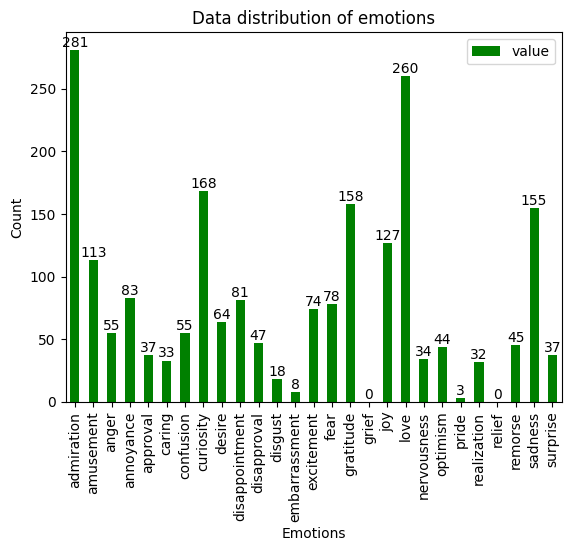
\includegraphics[width=\columnwidth]{figs/emotion_count.png}
% \caption{Distribution of our dataset per emotion. Note that our dataset doesn't include \textit{grief} and \textit{relief}.}
% \label{fig:emotion_count}
% \end{figure}


\end{document}


